\chapter{ΕΚΤΙΜΗΣΗ ΡΥΘΜΩΝ ΤΑΛΑΝΤΩΣΗΣ ΑΠΟ ΔΕΔΟΜΕΝΑ ΔΙΑΤΑΡΑΧΩΝ}
\label{chap:ringdown-analysis}

% Τα τμήματα του preliminary report είναι ανεξάρτητα αρχεία, ενώ το αρχικό
% IEEE report στο PreliminaryInvestigation/ παραμένει ανέπαφο.
\begingroup
\newcommand{\preliminaryfigurepath}{PreliminaryInvestigation/}
\newcommand{\ieeeThirtyNinePathanalysis}{IEEE39/analysis/}
\newif\ifkundursystemanalysis
\section{Εισαγωγή}

Στην παρούσα ενότητα εξετάζεται η εφαρμογή της μεθόδου ταυτοποίησης MP σε αποκρίσεις διαταραχών που προκύπτουν από δυναμικές προσομοιώσεις στο περιβάλλον \textenglish{\textit{PowerFactory}}. Η μεθοδολογία εφαρμόζεται σε χρονοσειρές τάσης ($V$), ρεύματος ($I$), ενεργού ($P$) και άεργου ($Q$) ισχύος, μετά από κατάλληλη προεπεξεργασία, με στόχο την εξαγωγή και τον χαρακτηρισμό των κυρίαρχων ρυθμών ταλάντωσης και την αξιολόγηση της ποιότητας της ανακατασκευής των σημάτων.

Η διερεύνηση πραγματοποιείται σε δύο ΣΗΕ διαφορετικής κλίμακας και πολυπλοκότητας, στο \textenglish{\textit{Kundur Two-Area System}}~\cite{kundur1994} και στο \textenglish{\textit{IEEE 39-Bus System}}~\cite{digsilent39,pai1989}. Με αυτόν τον τρόπο, η αναφορά δεν περιορίζεται μόνο σε ένα απλό σύστημα αναφοράς, αλλά επιτρέπει τη συγκριτική αξιολόγηση της συμπεριφοράς της μεθόδου ως προς την αναγνώριση \textenglish{\textit{inter-area}} και \textenglish{\textit{intra-area}} ρυθμών ταλάντωσης.

\subsection{Εξεταζόμενα Συστήματα}

Για τη μελέτη και την επαλήθευση των αλγορίθμων εκτίμησης και συσταδοποίησης ρυθμών ταλάντωσης, το σύστημα δοκιμής 2 Περιοχών-4 Γεννητριών του Kundur (\textenglish{\textit{Kundur Two-Area 4-Generator Benchmark System}}) αποτελεί διεθνές σύστημα αναφοράς. Το συγκεκριμένο σύστημα αποτελείται από δύο περιοχές που συνδέονται μέσω μιας διπλής ασθενούς διασυνδετικής γραμμής και εμφανίζει καθαρά διακριτούς τοπικούς ρυθμούς ταλάντωσης εντός κάθε περιοχής~\cite{kundur1994,klein1991interarea}. Το μονογραμμικό του διάγραμμα παρουσιάζεται στο Σχήμα~\ref{fig:examined-kundur-system}.

\begin{figure}[htbp]
    \centering
    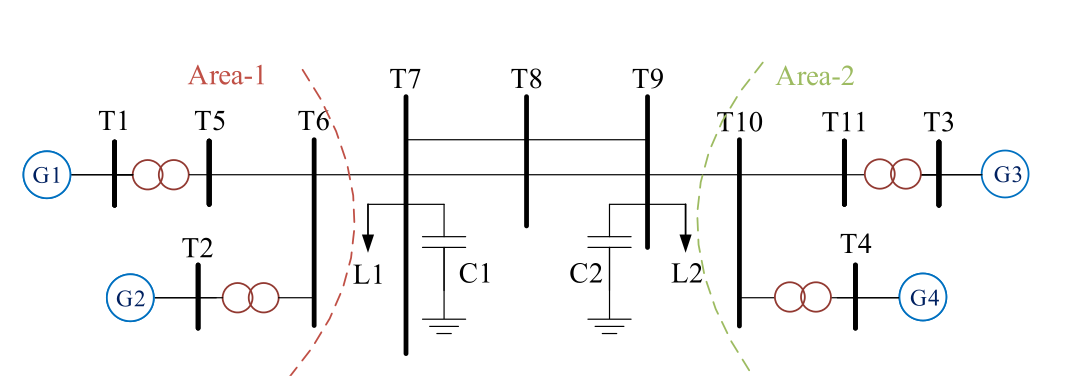
\includegraphics[width=0.92\textwidth]{images/system_figures/kundur_two_area_from_estimation2021.png}
    \caption{Μονογραμμικό διάγραμμα του \textenglish{\textit{Kundur Two-Area System}}~\cite{estimation2021}.}
    \label{fig:examined-kundur-system}
\end{figure}

Το πρότυπο σύστημα \textenglish{\textit{IEEE 39-Bus}} (\textenglish{\textit{New England Power System}}) αποτελεί ευρέως αποδεκτό σύστημα αναφοράς για μελέτες δυναμικής ευστάθειας και ταλαντώσεων ευρείας περιοχής. Αποτελείται από 39 ζυγούς, 10 γεννήτριες, εκ των οποίων η μία αναπαριστά ισοδύναμο διασύνδεσης μεγάλης έκτασης, 19 φορτία και 46 γραμμές μεταφοράς/μετασχηματιστές. Το σύστημα εμφανίζει τοπικούς και διασυνδετικούς ρυθμούς ταλάντωσης, καθιστώντας το κατάλληλο για την αξιολόγηση και σύγκριση της ακρίβειας των αλγορίθμων συσταδοποίησης υπό διαφορετικά σενάρια διείσδυσης ΑΠΕ και τύπων φορτίου~\cite{digsilent39,estimation2021,alzahrani2020dynamic}. Το μονογραμμικό του διάγραμμα και η διαίρεσή του σε τρεις περιοχές παρουσιάζονται στο Σχήμα~\ref{fig:examined-ieee39-system}.

Η κατάτμηση αυτή ομαδοποιεί τις γεννήτριες σύμφωνα με την ηλεκτρική τους θέση και τη συνεκτική δυναμική συμπεριφορά που αναμένεται να εμφανίζουν. Ειδικότερα, στην Περιοχή~1 εντάσσονται οι γεννήτριες $G_1$, $G_8$, $G_9$ και $G_{10}$, στην Περιοχή~2 οι $G_2$ και $G_3$, ενώ στην Περιοχή~3 οι $G_4$--$G_7$. Με τον διαχωρισμό αυτό, οι εκτιμώμενοι ρυθμοί μπορούν να εξετάζονται τόσο ανά περιοχή ελέγχου όσο και συνολικά για ολόκληρο το σύστημα.

Η διάκριση των περιοχών είναι ιδιαίτερα χρήσιμη για τη φυσική ερμηνεία των αποτελεσμάτων. Ταλαντώσεις μεταξύ γεννητριών της ίδιας περιοχής συνδέονται κυρίως με τοπικούς ρυθμούς, ενώ η συνεκτική κίνηση μιας ομάδας γεννητριών έναντι μιας άλλης χαρακτηρίζει διασυνδετικούς ρυθμούς. Συνεπώς, η χωρική πληροφορία του Σχήματος~\ref{fig:examined-ieee39-system} αξιοποιείται στη συνέχεια για την αξιολόγηση της ικανότητας των μεθόδων εκτίμησης και συσταδοποίησης να ανακτούν τις διαφορετικές μορφές ταλαντωτικής συμπεριφοράς.

\begin{figure}[htbp]
    \centering
    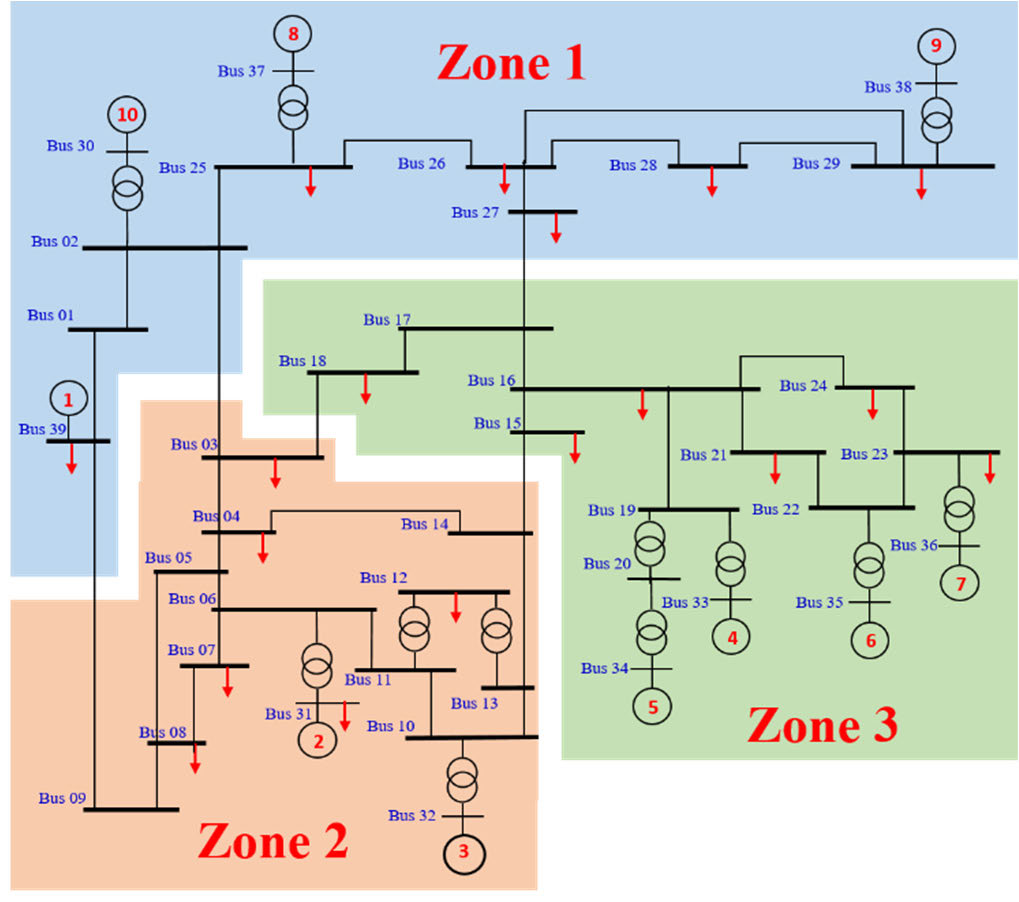
\includegraphics[width=0.82\textwidth]{images/system_figures/ieee39_three_zones_alzahrani2020.jpg}
    \caption{Μονογραμμικό διάγραμμα και διαίρεση του \textenglish{\textit{IEEE 39-Bus System}} σε τρεις περιοχές~\cite{alzahrani2020dynamic}.}
    \label{fig:examined-ieee39-system}
\end{figure}
\FloatBarrier


\kundursystemanalysistrue
\section{Ανάλυση του Συστήματος \textenglish{Kundur Two-Area}}
\subsection{Διαδικασία Παραγωγής Δεδομένων}
\ifkundursystemanalysis

Το πρώτο βήμα περιελάμβανε την εισαγωγή του συστήματος στο περιβάλλον του \textenglish{\textit{PowerFactory}} για τη δημιουργία των απαραίτητων χρονοσειρών. Συγκεκριμένα, εκτελέστηκε προσομοίωση \textenglish{RMS}, αφού πρώτα επιλύθηκε πρόβλημα ροής φορτίου για τον καθορισμό των αρχικών συνθηκών \textenglish{(Initial Conditions)}. Η συνολική διάρκεια της προσομοίωσης ορίστηκε στα $50$ s, με χρονικό βήμα ολοκλήρωσης (\textenglish{\textit{step size}}) $0.01$ s, επιτρέποντας την πλήρη καταγραφή της απόκρισης μετά την διαταραχή (\textenglish{\textit{ringdown}}) καθώς το σύστημα τείνει προς ένα νέο σημείο ισορροπίας. Για την παρακολούθηση των φαινομένων, εξήχθησαν οι μεταβλητές τάσης ($V$), ρεύματος ($I$), ενεργού ($P$) και άεργου ($Q$) ισχύος για καθεμία από τις γεννήτριες του συστήματος.

Ως συμβάν διαταραχής (\textenglish{\textit{event}}) για τη διέγερση των ηλεκτρομηχανικών ταλαντώσεων, ορίστηκε η προσωρινή αποσύνδεση της διασυνδετικής γραμμής \textenglish{07a\textendash{07b}}, η οποία συνδέει τις δύο περιοχές του συστήματος. Η γραμμή αποσυνδέθηκε τη χρονική στιγμή $t=0$~s και παρέμεινε εκτός λειτουργίας για $0.1$~s, πριν από την αυτόματη επανασύνδεσή της στο $t=0.1$~s. Η συγκεκριμένη διαταραχή ακολουθεί τη μεθοδολογία της βιβλιογραφίας για την παραγωγή αποκρίσεων \textenglish{\textit{ringdown}}, σύμφωνα με την οποία η προσωρινή αποσύνδεση μίας από τις δύο διασυνδετικές γραμμές του συστήματος και η επανασύνδεσή της μετά από $0.1$~s διεγείρει τους ρυθμούς ταλάντωσης του συστήματος~\cite{estimation2021}.

\subsubsection{Προεπεξεργασία Σημάτων.}
Πριν την εφαρμογή του αλγορίθμου MP, τα πρωτογενή δεδομένα του \textenglish{\textit{PowerFactory}} υποβλήθηκαν σε απαραίτητη ψηφιακή επεξεργασία (μέσω της γλώσσας Python), προκειμένου να εξασφαλιστεί η αξιοπιστία της ταυτοποίησης. Τα στάδια της προεπεξεργασίας περιελάμβαναν:

\begin{enumerate}
    \item \textbf{Αποκοπή Χρονοσειρών:} Μετά την εφαρμογή και την άρση της διαταραχής, η άμεση μεταβατική απόκριση μπορεί να επηρεάζεται από μη γραμμικότητες, υποβαθμίζοντας την ακρίβεια της ταυτοποίησης των ρυθμών ταλάντωσης~\cite{sfetkos2024measurement}. Για τον περιορισμό της επίδρασης της αρχικής μεταβατικής φάσης, απορρίφθηκαν τα δεδομένα έως $t=0.2$~s και η ανάλυση εφαρμόστηκε στο τμήμα της απόκρισης \textenglish{\textit{ringdown}} που διατηρήθηκε.
    \item \textbf{Αφαίρεση Γραμμικής Τάσης (\textenglish{\textit{Detrending}}):} Αφαιρέθηκε η βέλτιστη γραμμική τάση που περιλαμβάνει τη \textenglish{DC} συνιστώσα και τυχόν κλίση του σήματος.
    \item \textbf{Φιλτράρισμα:} Εφαρμόστηκε βαθυπερατό φίλτρο (\textenglish{\textit{Low-Pass}}) με συχνότητα αποκοπής $f_{c} = 10$ Hz για την απομάκρυνση υψίσυχνου θορύβου και συνιστωσών εκτός του πεδίου ενδιαφέροντος.
\end{enumerate}

\subsubsection{Στάδιο Ελέγχου και Φιλτραρίσματος των Δεδομένων.}
\label{subsec:data_screening}

Μετά την εξαγωγή των εκτιμώμενων ρυθμών από τις επιμέρους μεθόδους αναγνώρισης, εφαρμόστηκε στάδιο φιλτραρίσματος (\textenglish{\textit{data screening}}) των δεδομένων, με στόχο τη διασφάλιση της καταλληλότητάς τους για τη διαδικασία συσταδοποίησης. Το στάδιο αυτό δεν μετέβαλε τη διαδικασία υπολογισμού των ρυθμών, αλλά λειτούργησε ως βήμα προεπεξεργασίας πριν από την εφαρμογή των τεχνικών συσταδοποίησης. Η ανάγκη για φιλτράρισμα προέκυψε από το γεγονός ότι οι επιμέρους εκτιμήσεις που παράγονται από την ανάλυση MP ενδέχεται να περιλαμβάνουν τιμές που δεν σχετίζονται με πραγματικούς ηλεκτρομηχανικούς ρυθμούς ταλάντωσης, αλλά οφείλονται σε θόρυβο, αριθμητικές αβεβαιότητες ή μη φυσικούς ρυθμούς.

Σύμφωνα με τη σχετική βιβλιογραφία, οι \textenglish{\textit{inter-area}} ρυθμοί ταλάντωσης του \textenglish{\textit{Kundur Two-Area System}} εμφανίζονται στην περιοχή από $0.1$~Hz έως $0.7$~Hz, ενώ οι \textenglish{\textit{intra-area}} ρυθμοί ταλάντωσης εντοπίζονται στην περιοχή από $0.7$~Hz έως $2.0$~Hz~\cite{estimation2021}. Συνεπώς, διατηρήθηκαν μόνο οι εκτιμήσεις με συχνότητα εντός του διαστήματος $[0.1,\,2.0]$~Hz και με αρνητικό ρυθμό απόσβεσης που να ικανοποιεί το όριο $\sigma \leq -10^{-3}$. Έτσι προέκυψε ένα καθαρό σύνολο δεδομένων, κατάλληλο για την εφαρμογή των τεχνικών συσταδοποίησης που αξιοποιήθηκαν στη συνέχεια της ανάλυσης.

\else
Παρόμοια με την περίπτωση του \textenglish{\textit{Kundur Two-Area System}}, εκτελέστηκε προσομοίωση \textenglish{RMS} διάρκειας $50$ s με χρονικό βήμα $0.01$ s και εξήχθησαν οι μεταβλητές $V$, $I$, $P$ και $Q$ για κάθε γεννήτρια. Ως διαταραχή εφαρμόστηκε αύξηση της ενεργού ισχύος $P$ του φορτίου $3$ (\textenglish{\textit{Load 03}}) κατά $2\%$ τη χρονική στιγμή $t=0$ s~\cite{digsilent39,sfetkos2024measurement}.

Στα παραγόμενα σήματα εφαρμόστηκαν τα ίδια στάδια προεπεξεργασίας και φιλτραρίσματος με την περίπτωση του συστήματος Kundur. Οι ρυθμοί αναφοράς του \textenglish{\textit{IEEE 39-Bus System}} βρίσκονται επίσης εντός της περιοχής $[0.1,\,2.0]$~Hz~\cite{sarkar2024drga} και, επομένως, χρησιμοποιήθηκαν τα ίδια κριτήρια διατήρησης των εκτιμήσεων.
\fi

\subsection{Εφαρμογή της Μεθόδου Matrix Pencil}
\ifkundursystemanalysis
Η ανάλυση των αποκρίσεων διαταραχών μέσω τεχνικών ταυτοποίησης συστήματος αποτελεί μια μέθοδο για την παρακολούθηση της δυναμικής ευστάθειας \cite{modal2018}. Η διαδικασία της ταυτοποίησης βασίστηκε στην ανάλυση των προεπεξεργασμένων σημάτων $V$, $I$, $P$ και $Q$ μέσω του αλγορίθμου MP. Σύμφωνα με τις απαιτήσεις της διερεύνησης, η μέθοδος εφαρμόστηκε με δύο διαφορετικές προσεγγίσεις για τον καθορισμό της τάξης $n$ του συστήματος.

\begin{enumerate}
    \item \textbf{Καθορισμένη Τάξη:} Χρησιμοποιήθηκαν σταθερές τιμές τάξης $n \in \{2, 4, 6\}$.
    \item \textbf{Αυτόματος Καθορισμός Τάξης:} Για τον αυτόματο καθορισμό της τάξης του μοντέλου εφαρμόστηκε ο αλγόριθμος της~\cite{estimation2021}. Εξετάστηκαν τρία διαφορετικά επίπεδα ανοχής, $\tau \in \{1, 0.1, 0.01\}$. Ο αλγόριθμος επιλέγει αυτόματα την τάξη του μοντέλου μέσω μιας διαδικασίας διαδοχικής βελτίωσης της ανακατασκευής του σήματος. Στο πλαίσιο αυτό, η τάξη αυξανόταν μέχρι η μεταβολή του συντελεστή $R^2$ μεταξύ δύο διαδοχικών ανακατασκευών να γίνει μικρότερη απο $\tau$.
\end{enumerate}
\else
Παρόμοια με την περίπτωση του συστήματος Kundur, η μέθοδος MP εφαρμόστηκε στα προεπεξεργασμένα σήματα $V$, $I$, $P$ και $Q$, τόσο με καθορισμένη όσο και με αυτόματα επιλεγόμενη τάξη. Η μόνη διαφοροποίηση ήταν ότι, εκτός από τις σταθερές τιμές $n\in\{2,4,6\}$, εξετάστηκε επιπλέον η τιμή $n=8$, λόγω του μεγαλύτερου πλήθους ηλεκτρομηχανικών ρυθμών του \textenglish{\textit{IEEE 39-Bus System}}~\cite{sarkar2024drga}. Για τον αυτόματο καθορισμό της τάξης χρησιμοποιήθηκαν τα ίδια επίπεδα ανοχής $\tau\in\{1,0.1,0.01\}$.
\fi

\subsection{Μαθηματική Ανακατασκευή και Πιστότητα}
\ifkundursystemanalysis
Για κάθε σενάριο ταυτοποίησης εξήχθησαν οι παράμετροι των αναγνωρισμένων ρυθμών ταλάντωσης: το πλάτος ($A_{i}$), ο ρυθμός απόσβεσης ($\sigma_{i}$), η συχνότητα ($f_{i}$ σε Hz) και η φάση ($\varphi_{i}$). Η μαθηματική ανακατασκευή του σήματος $\hat{y}(t)$ πραγματοποιήθηκε μέσω της σχέσης:

\begin{equation}
\hat{y}(t)=\sum_{i=1}^{n}A_{i}e^{\sigma_{i}t}\cos(2\pi f_{i}t+\varphi_{i})
\label{eq:reconstruction}
\end{equation}

Η πιστότητα της ανακατασκευής αξιολογήθηκε μέσω του συντελεστή προσδιορισμού $R^{2}$ και της τετραγωνικής ρίζας του μέσου τετραγωνικού σφάλματος (RMSE), οι οποίοι υπολογίζονται αντίστοιχα από τις σχέσεις:

\begin{equation}
R^2=1-\frac{\displaystyle\sum_{k=1}^{N}\left(y_k-\hat{y}_k\right)^2}
{\displaystyle\sum_{k=1}^{N}\left(y_k-\bar{y}\right)^2}
\label{eq:reconstruction_r2}
\end{equation}

\begin{equation}
\mathrm{RMSE}=\sqrt{\frac{1}{N}\sum_{k=1}^{N}\left(y_k-\hat{y}_k\right)^2}
\label{eq:reconstruction_rmse}
\end{equation}

όπου $y_k$ και $\hat{y}_k$ είναι αντίστοιχα η πραγματική και η ανακατασκευασμένη τιμή του σήματος στο $k$-οστό δείγμα, $\bar{y}$ είναι η μέση τιμή του πραγματικού σήματος και $N$ το συνολικό πλήθος των δειγμάτων. Τιμές του $R^2$ κοντά στη μονάδα και μικρές τιμές του RMSE υποδηλώνουν υψηλή πιστότητα ανακατασκευής. Η διαδικασία αυτή εξασφαλίζει ότι οι ταυτοποιημένοι ρυθμοί ταλάντωσης αντιπροσωπεύουν με ακρίβεια τη φυσική απόκριση των εξεταζόμενων συστημάτων και δεν αποτελούν μαθηματικά σφάλματα της προσέγγισης.
\else
Η ανακατασκευή των σημάτων και η αξιολόγηση της πιστότητάς της πραγματοποιήθηκαν παρόμοια με την περίπτωση του συστήματος Kundur, μέσω των~(\ref{eq:reconstruction})-(\ref{eq:reconstruction_rmse}).
\fi



\subsection{Αποτελέσματα και Γραφικές Παραστάσεις}

\subsubsection{Απεικόνιση Ρυθμού Απόσβεσης και Συχνότητας}
\ifkundursystemanalysis
\label{sec:modal_and_reconstruction_plots}
\fi
Ως αποτέλεσμα της εφαρμογής του αλγορίθμου MP, ελήφθησαν τα διαγράμματα της παρούσας παραγράφου, στα οποία παρουσιάζεται η κατανομή των ιδιοτιμών στο μιγαδικό επίπεδο για τα μετρούμενα μεγέθη των γεννητριών των συστημάτων. Συγκεκριμένα, στον οριζόντιο άξονα παρουσιάζεται ο ρυθμός απόσβεσης, ο οποίος αποτελεί το πραγματικό μέρος των ιδιοτιμών, ενώ στον κατακόρυφο άξονα η συχνότητα ταλάντωσης σε Hz.


\ifkundursystemanalysis
\begin{figure}[H]
    \centering
    \includegraphics[width=0.94\textwidth,height=0.82\textheight,keepaspectratio]{\preliminaryfigurepath plots/modal_maps/pdf/All_Generators_Grid.pdf}
    \caption{Κατανομή ιδιοτιμών (\textit{Πραγματικό Μέρος έναντι Συχνότητας}) για τις γεννήτριες $G_1$-$G_4$ του \textenglish{\textit{Kundur Two-Area System}}.}
    \label{fig:poles_distribution_all_kundur}
\end{figure}
\else
\begin{figure}[!htbp]
    \centering
    \includegraphics[width=0.94\textwidth,height=0.82\textheight,keepaspectratio]{\ieeeThirtyNinePathanalysis/Load03_Pplus2_50s_0.2_to_end_reset/plots/modal_maps/pdf/All_Generators_Grid.pdf}
    \caption{Κατανομή ιδιοτιμών (\textit{Πραγματικό Μέρος έναντι Συχνότητας}) για τις γεννήτριες $G_1$-$G_{10}$ του \textenglish{\textit{IEEE 39-Bus System}}.}
    \label{fig:poles_distribution_all_ieee39}
\end{figure}
\fi


\ifkundursystemanalysis
Στο Σχήμα~\ref{fig:poles_distribution_all_kundur} αποτυπώνεται η κατανομή των ταυτοποιημένων ιδιοτιμών για τις τέσσερις γεννήτριες του \textenglish{\textit{Kundur Two-Area System}} ($G_1$-$G_4$).
\else
Στο Σχήμα~\ref{fig:poles_distribution_all_ieee39} παρουσιάζεται η κατανομή των ιδιοτιμών για τις δέκα γεννήτριες του \textenglish{\textit{IEEE 39-Bus System}}.
\fi
Το σύνολο των ηλεκτρομηχανικών ιδιοτιμών εντοπίζεται στο αριστερό ημιεπίπεδο ($\sigma$ < 0), υποδεικνύοντας τη θετική απόσβεση των ταλαντώσεων.
Ακόμα, καταγράφονται στον οριζόντιο άξονα και ιδιοτιμές με μηδενική συχνότητα, οι οποίες δεν αντιστοιχούν σε κύριους ρυθμούς ταλάντωσης, αλλά σε ρυθμούς που σχετίζονται με τα συστήματα ελέγχου, καθώς και σε ψευδείς ρυθμούς \textenglish{(spurious modes)}.

\subsubsection{Αξιολόγηση Πιστότητας Ανακατασκευής}
Για την επαλήθευση της εγκυρότητας των ταυτοποιημένων ρυθμών που εξήχθησαν στην προηγούμενη ενότητα, πραγματοποιήθηκε μαθηματική ανακατασκευή των σημάτων στο πεδίο του χρόνου. Εξετάστηκαν οι επιμέρους προσεγγίσεις σταθερής τάξης $n$ και ανοχής $\tau$ και, για κάθε σήμα, επιλέχθηκε η μέθοδος που απέδωσε τη μεγαλύτερη τιμή του συντελεστή προσδιορισμού $R^2$. Στο
\ifkundursystemanalysis
Σχήμα~\ref{fig:best_recon_g1_kundur}
\else
Σχήμα~\ref{fig:best_recon_g9_ieee39}
\fi
παρουσιάζεται ένα αντιπροσωπευτικό παράδειγμα, στο οποίο συγκρίνονται τα αρχικά φιλτραρισμένα σήματα με τις αντίστοιχες ανακατασκευασμένες κυματομορφές που προέκυψαν από τη μέθοδο MP.

\ifkundursystemanalysis
\begin{figure}[H]
    \centering
    \captionsetup{font=small,skip=4pt}
    \includegraphics[width=0.96\textwidth,height=0.72\textheight,keepaspectratio]{\preliminaryfigurepath stats/pdf/10_best_reconstruction_g1_2x2.pdf}
    \caption{Βέλτιστη μαθηματική ανακατασκευή των σημάτων ($V, I, P, Q$) για τη γεννήτρια $G_1$ του \textenglish{\textit{Kundur Two-Area System}} με βάση τον μέγιστο συντελεστή προσδιορισμού $R^2$.}
    \label{fig:best_recon_g1_kundur}
\end{figure}
\else
\begin{figure}[H]
    \centering
    \captionsetup{font=small,skip=4pt}
    \includegraphics[width=0.96\textwidth,height=0.72\textheight,keepaspectratio]{\ieeeThirtyNinePathanalysis/Load03_Pplus2_50s_0.2_to_end_reset/stats/pdf/10_best_reconstruction_g9_2x2.pdf}
    \caption{Βέλτιστη μαθηματική ανακατασκευή των σημάτων ($V, I, P, Q$) για τη γεννήτρια $G_{9}$ του \textenglish{\textit{IEEE 39-Bus System}} με βάση τον μέγιστο συντελεστή προσδιορισμού $R^2$.}
    \label{fig:best_recon_g9_ieee39}
\end{figure}
\fi

Όπως παρατηρείται στο αντιπροσωπευτικό παράδειγμα, επιτυγχάνεται εξαιρετική σύμπτωση μεταξύ των αρχικών και των ανακατασκευασμένων κυματομορφών. Αξίζει να σημειωθεί, ωστόσο, ότι η βέλτιστη ανακατασκευή δεν προκύπτει από μία καθολική επιλογή τάξης ή ανοχής, γεγονός που επιβεβαιώνει την αναγκαιότητα εξέτασης πολλαπλών προσεγγίσεων.

Τέλος, η ταύτιση των κυματομορφών αναλύεται στο χρονικό παράθυρο της γραμμικής συμπεριφοράς, δηλαδή για t > 0.2 s. Η υψηλή πιστότητα της ανακατασκευής επιβεβαιώνει την ορθή επιλογή του παραθύρου ανάλυσης, καθώς και την αποτελεσματικότητα της προεπεξεργασίας των σημάτων.

\FloatBarrier
\subsubsection{Ταυτοποίηση Κυρίαρχων Ρυθμών Ταλάντωσης}
\ifkundursystemanalysis
\label{subsec:overall_evaluation}

Η συνολική αξιολόγηση της δυναμικής του συστήματος πραγματοποιήθηκε με βάση τα διαγράμματα της Ενότητας \ref{sec:modal_and_reconstruction_plots} και το Διάγραμμα Φυσαλίδων (\textenglish{\textit{Bubble Map}}) του Σχήματος~\ref{fig:bubble_map_kundur}. Με τον τρόπο αυτό αποτυπώθηκαν συνολικά η συχνότητα, η απόσβεση και η ενέργεια των ταυτοποιημένων ρυθμών ταλάντωσης.
Για την αποτύπωση της σχετικής σημασίας κάθε ρυθμού ταλάντωσης στα Διαγράμματα Φυσαλίδων , υπολογίστηκε η ενέργεια κάθε ρυθμού ταλάντωσης σύμφωνα με:
\begin{equation}
\omega_i = 2\pi f_i
\end{equation}
\begin{equation}
\label{eq:pole_energy}
E_i = \frac{1}{2}\omega_i^2 \alpha_i^2
\end{equation}
όπου $f_i$ είναι η συχνότητα και $\alpha_i$ το πλάτος του $i$-οστού ρυθμού. Το μέγεθος κάθε φυσαλίδας είναι ανάλογο της ποσότητας $E_i$ \cite{sfetkos2024measurement}.

Η συγκεκριμένη απεικόνιση παρέχει τη συνολικότερη εικόνα της ταυτοποίησης και επιβεβαιώνει τα ευρήματα που παρουσιάστηκαν στην Ενότητα \ref{sec:modal_and_reconstruction_plots}. Παρατηρείται συγκέντρωση εκτιμήσεων σε τρεις βασικές περιοχές συχνοτήτων: πολύ κοντά στο $0$ Hz, στην περιοχή $0.5-0.6$ Hz και γύρω από το $1.1$ Hz. Η πρώτη περιοχή συνδέεται κυρίως με αργές μη ταλαντωτικές συνιστώσες και με ψευδείς ρυθμούς της μεθόδου, ενώ οι υπόλοιπες αντιστοιχούν σε κυρίαρχους ρυθμούς ταλάντωσης του συστήματος.
% Παράλληλα, η κατανομή των ιδιοτιμών ως προς τον ρυθμό απόσβεσης $\sigma$ δείχνει ότι οι ταλαντώσεις εμφανίζουν γενικά θετική απόσβεση, καθώς τα περισσότερα σημεία εντοπίζονται στο αριστερό ημιεπίπεδο.

Για το σύστημα \textenglish{\textit{Kundur Two-Area}}, η ποσοτική αποτύπωση των κυρίαρχων ρυθμών ταλάντωσης παρουσιάζεται στον Πίνακα~\ref{tab:summary_modes}. Οι τιμές του πίνακα επιλέχθηκαν με βάση τη μέγιστη ενέργεια στις περιοχές συχνοτήτων $0.4-0.6$~Hz και $1.0-1.1$~Hz, σύμφωνα με την~(\ref{eq:pole_energy}). Στο Σχήμα~\ref{fig:bubble_map_kundur}, οι μεγαλύτερες φυσαλίδες στην περιοχή των $0.54$~Hz εμφανίζονται κυρίως στα σήματα ενεργού ισχύος των γεννητριών $G_3$ και $G_4$, αναδεικνύοντας την υψηλή ενεργειακή συμμετοχή του κυρίαρχου διασυνδετικού ρυθμού.


\raggedbottom
\begin{figure}[H]
    \centering
    \includegraphics[width=0.98\textwidth,keepaspectratio,trim=15pt 65pt 10pt 35pt,clip]{\preliminaryfigurepath stats/pdf/5_bubble_map.pdf}
    \caption{Διαγράμματα Φυσαλίδων-Συγκεντρωτική απεικόνιση συχνότητας, απόσβεσης και ενέργειας των ταυτοποιημένων ρυθμών ταλάντωσης.}
    \label{fig:bubble_map_kundur}
\end{figure}

Σημαντική ενέργεια παρουσιάζουν επίσης οι εκτιμήσεις στην περιοχή $1.0-1.1$~Hz, ιδιαίτερα στα σήματα ενεργού ισχύος, οι οποίες αντιστοιχούν στους τοπικούς ρυθμούς του συστήματος. Αντίθετα, οι συνιστώσες πολύ κοντά στα $0$~Hz εμφανίζουν γενικά μικρότερες φυσαλίδες και, συνεπώς, χαμηλότερη ενέργεια, γεγονός που υποστηρίζει τον διαχωρισμό τους από τους κυρίαρχους ηλεκτρομηχανικούς ρυθμούς. Οι τοπικοί ρυθμοί εμφανίζονται επιπλέον με μεγαλύτερες απόλυτες τιμές απόσβεσης σε σχέση με τον διασυνδετικό ρυθμό.

\else
Η συνολική αξιολόγηση πραγματοποιήθηκε παρόμοια με την περίπτωση του συστήματος Kundur, με βάση την κατανομή των εκτιμώμενων ρυθμών και το Διάγραμμα Φυσαλίδων του Σχήματος~\ref{fig:bubble_map_ieee39}. Η ενέργεια των ταυτοποιημένων ρυθμών υπολογίστηκε σύμφωνα με την~(\ref{eq:pole_energy}).

\begin{figure}[!htbp]
    \centering
    \includegraphics[width=0.94\textwidth,height=0.64\textheight,keepaspectratio,trim=20pt 260pt 15pt 100pt,clip]{\ieeeThirtyNinePathanalysis/Load03_Pplus2_50s_0.2_to_end_reset/stats/pdf/5_bubble_map_single_panel.pdf}
    \caption{Διαγράμματα Φυσαλίδων-Συγκεντρωτική απεικόνιση συχνότητας, απόσβεσης και ενέργειας των ταυτοποιημένων ρυθμών ταλάντωσης.}
    \label{fig:bubble_map_ieee39}
\end{figure}


Αξίζει να σημειωθεί ότι στο \textenglish{\textit{IEEE 39-Bus System}} η αντίστοιχη ποσοτική ερμηνεία δεν είναι εξίσου άμεση, λόγω της μεγαλύτερης πολυπλοκότητας του συστήματος. Για τον λόγο αυτό, η αξιολόγηση του \textenglish{\textit{IEEE 39-Bus System}} βασίζεται κυρίως στις συνολικές γραφικές απεικονίσεις και στη συγκριτική ερμηνεία των αποτελεσμάτων.
\fi

\ifkundursystemanalysis
\begin{table}[h]
\centering
\caption{Σύνοψη Κυρίαρχων Ρυθμών Ταλάντωσης με Κριτήριο τη Μέγιστη Ενέργεια}
\label{tab:summary_modes}
\resizebox{\textwidth}{!}{%
\begin{tabular}{cccc | ccc}
\toprule
\multicolumn{4}{c}{\textbf{Inter-area ρυθμός ταλάντωσης ($0.4-0.6$ Hz)}} & \multicolumn{3}{c}{\textbf{Intra-area ρυθμοί ταλάντωσης ($1.0-1.1$ Hz)}} \\
\cmidrule(lr){1-4}\cmidrule(lr){5-7}
\textbf{Γεν.} & \textbf{σήμα} & \textbf{$f$ [Hz]} & \textbf{$\sigma$ [rad/s]} & \textbf{σήμα} & \textbf{$f$ [Hz]} & \textbf{$\sigma$ [rad/s]} \\
\midrule
    G1 & P & 0.543 & -0.125 & P & 1.043 & -0.838 \\
    & Q & 0.543 & -0.126 & Q & 1.038 & -0.766 \\
    & V & 0.542 & -0.131 & V & $-$ & $-$ \\
    & I & 0.543 & -0.125 & I & 1.040 & -0.799 \\
    \midrule
    G2 & P & 0.539 & -0.144 & P & 1.059 & -0.773 \\
    & Q & 0.543 & -0.127 & Q & 1.079 & -0.664 \\
    & V & 0.543 & -0.129 & V & $-$ & $-$ \\
    & I & 0.543 & -0.126 & I & 1.052 & -0.776 \\
    \midrule
    G3 & P & 0.544 & -0.136 & P & 1.087 & -0.697 \\
    & Q & 0.543 & -0.124 & Q & 1.025 & -0.848 \\
    & V & 0.543 & -0.130 & V & 1.017 & -1.066 \\
    & I & 0.544 & -0.137 & I & 1.088 & -0.727 \\
    \midrule
    G4 & P & 0.543 & -0.127 & P & 1.091 & -0.849 \\
    & Q & 0.543 & -0.131 & Q & $-$ & $-$ \\
    & V & 0.543 & -0.130 & V & 1.027 & -0.796 \\
    & I & 0.543 & -0.127 & I & 1.094 & -0.817 \\
\bottomrule
\end{tabular}
}
\end{table}
\fi

\subsubsection{Αξιολόγηση των Εκτιμήσεων μέσω του Δείκτη \textit{MAD}}
\ifkundursystemanalysis
\label{subsec:mad_evaluation}

Μετά το στάδιο ελέγχου και φιλτραρίσματος των δεδομένων, πραγματοποιήθηκε ποσοτική
αξιολόγηση των εκτιμώμενων ρυθμών ταλάντωσης που προέκυψαν από τη μέθοδο \textenglish{\textit{MP}} ως προς
τους θεωρητικούς ρυθμούς ταλάντωσης των εξεταζόμενων συστημάτων. Για τον σκοπό αυτό χρησιμοποιήθηκε
ο δείκτης \textenglish{\textit{MAD}}~\cite{modal2018}.

\begin{equation}
\mathrm{MAD}_i = \mathrm{median}\left(\left| \hat{\lambda}_{i,j} - \lambda_i \right|\right)
\label{eq:mad_definition}
\end{equation}
όπου \(\hat{\lambda}_{i,j}\) είναι η \(j\)-οστή εκτίμηση της ιδιοτιμής του \(i\)-οστού
ρυθμού ταλάντωσης και \(\lambda_i\) η αντίστοιχη θεωρητική ιδιοτιμή αναφοράς.

Ως ρυθμοί αναφοράς λήφθηκαν οι τρεις κυρίαρχοι ρυθμοί ταλάντωσης του
συστήματος Kundur~\cite{estimation2021}, οι οποίοι παρουσιάζονται στον
Πίνακα~\ref{tab:kundur_reference_modes}. Ο πρώτος ρυθμός ταλάντωσης αντιστοιχούσε στον \textenglish{\textit{inter-area}}
ρυθμό ταλάντωσης του συστήματος, ενώ οι δύο επόμενοι στους \textenglish{\textit{intra-area}} ρυθμούς ταλάντωσης των δύο περιοχών.


\begin{table}[!htbp]
\centering
\caption{Ρυθμοί αναφοράς του συστήματος Kundur Two-Area System.}
\label{tab:kundur_reference_modes}
\begin{tabular}{ccc}
\toprule
\textbf{ρυθμός ταλάντωσης} & \textbf{$f$ [Hz]} & \textbf{$\sigma$ [rad/s]} \\
\midrule
\textenglish{\textit{Inter-area}}   & 0.540 & -0.127 \\
\textenglish{\textit{Intra-area}} 1 & 1.083 & -0.603 \\
\textenglish{\textit{Intra-area}} 2 & 1.119 & -0.631 \\
\bottomrule
\end{tabular}
\end{table}
\else
Η αξιολόγηση πραγματοποιήθηκε παρόμοια με την περίπτωση του συστήματος Kundur, μέσω του δείκτη \textenglish{\textit{MAD}} της~(\ref{eq:mad_definition}). Ως ρυθμοί αναφοράς λήφθηκαν οι εννέα κυρίαρχοι ρυθμοί που παρουσιάζονται στον Πίνακα~\ref{tab:ieee39_reference_modes}~\cite{sarkar2024drga}.

\begin{table}[!htbp]
\centering
\caption{Ρυθμοί αναφοράς του συστήματος IEEE 39-Bus.}
\label{tab:ieee39_reference_modes}
\resizebox{\textwidth}{!}{%
\begin{tabular}{cccccc}
\toprule
\textbf{ρυθμός ταλάντωσης} & \textbf{$f$ [Hz]} & \textbf{$\sigma$ [rad/s]}  & \textbf{γεννήτριες} & \textbf{περιοχές} & \textbf{τύπος} \\
\midrule
ρυθμός ταλάντωσης 1 & 0.6062 & -0.0800  & 1$-$9 vs. 10 & 1-3 &  Inter-area\\
ρυθμός ταλάντωσης 2 & 0.9497 & -0.1065  & 1, 8, 9 vs. 4, 5, 6, 7 & 1, 2 & Inter-area \\
ρυθμός ταλάντωσης 3 & 1.0312 & -0.2558  & 2, 3 vs. 4, 5 & 2, 3 & Inter-area\\
ρυθμός ταλάντωσης 4 & 1.1211 & -0.3373  & 2, 3 vs. 6, 7 &  2, 3 & Inter-area \\
ρυθμός ταλάντωσης 5 & 1.3155 & -0.4033  & 2 vs. 3 &  2 & Intra-area\\
ρυθμός ταλάντωσης 6 & 1.2851 & -0.3458  & 1 vs. 8, 9 & 1 & Intra-area\\
ρυθμός ταλάντωσης 7 & 1.4953 & -0.7033  & 4 vs. 5 & 3 & Intra-area\\
ρυθμός ταλάντωσης 8 & 1.5202 & -0.6010  & 5, 7 vs. 4, 6 & 3 & Intra-area\\
ρυθμός ταλάντωσης 9 & 1.5468 & -0.6376  & 1 vs. 8 & 1 & Intra-area\\
\bottomrule
\end{tabular}
}
\end{table}
\fi

\ifkundursystemanalysis
Για τον υπολογισμό του MAD χρησιμοποιήθηκαν οι εκτιμήσεις που παρέμειναν μετά το
στάδιο ελέγχου δεδομένων της Παραγράφου~\ref{subsec:data_screening}. Για κάθε μέθοδο συσταδοποίησης, κάθε τελική συστάδα αντιστοιχίζεται στο πλησιέστερο ρυθμό αναφοράς μέσω του
αντιπροσώπου της (κέντρο ή medoid) στο επίπεδο $(\sigma,\omega)$. Ο MAD κάθε ρυθμού ταλάντωσης είναι η διάμεσος των αποστάσεων
των εκτιμήσεων που ανήκουν στις συστάδες οι οποίες αντιστοιχίστηκαν σε αυτό. Με τον τρόπο
αυτό, ο δείκτης MAD παρείχε ένα συνοπτικό και ανθεκτικό μέτρο της απόκλισης των τελικών
εκτιμήσεων από τις θεωρητικές θέσεις των κυρίαρχων ρυθμών ταλάντωσης του συστήματος και τα βασικά αποτελέσματα των υπολογισμών συνοψίζονται στον Πίνακα~\ref{tab:mad_summary_kundur} τα οποία σχολιάζονται στην Ενότητα~\ref{sec:kundur-clustering-results}.




\begin{table}[!t]
\centering
\caption{MAD ανά μέθοδο συσταδοποίησης για το Kundur Two-Area System.}
\label{tab:mad_summary_kundur}
\begin{tabular}{ccccc}
\toprule
\textbf{ρυθμός ταλάντωσης} & \multicolumn{2}{c}{\textbf{k-Means}} & \multicolumn{2}{c}{\textbf{k-Medoids}} \\
\cmidrule(lr){2-3}\cmidrule(l){4-5}
 & \textbf{πλήθος} & \textbf{MAD} & \textbf{πλήθος} & \textbf{MAD} \\
\midrule
\textenglish{\textit{Inter-area}}   & 98 & 0.0190 & 98 & 0.0190 \\
\textenglish{\textit{Intra-area}} 1 & 45 & 0.2584 & 45 & 0.2584 \\
\textenglish{\textit{Intra-area}} 2 & 0  & $-$     & 0  & $-$     \\
\bottomrule
\end{tabular}
\end{table}
\else
Για το \textenglish{\textit{IEEE 39-Bus System}}, τα αποτελέσματα του δείκτη MAD παρουσιάζονται στον
Πίνακα~\ref{tab:mad_summary_ieee39} ανά ρυθμό αναφοράς. Για ρυθμούς ταλάντωσης χωρίς καμία
αντιστοιχισμένη εκτίμηση καταγράφεται πλήθος ίσο με μηδέν. Παρατηρείται ότι η καλύτερη
συμφωνία εμφανίζεται κυρίως για τους ρυθμούς ταλάντωσης~3 και~4, οι οποίοι παρουσιάζουν τις μικρότερες τιμές MAD. Αντίθετα, ο ρυθμός ταλάντωσης~1 συγκεντρώνει το μεγαλύτερο πλήθος εκτιμήσεων ($265$), όπως ήταν αναμενόμενο καθώς είναι παρατηρίσιμο από όλες τις περιοχές ελέγχου του συστήματος, αλλά και σαφώς μεγαλύτερη τιμή δείκτη \textenglish{\textit{MAD}} ($0.3437$). Σημειώνεται ότι, για το \textenglish{\textit{IEEE 39-Bus System}}, οι εκτιμήσεις κάθε περιοχής ελέγχου αντιστοιχίζονται μόνο στους ρυθμούς αναφοράς για τους οποίους η βιβλιογραφία υποδεικνύει συμμετοχή των αντίστοιχων γεννητριών~\cite{sarkar2024drga}. Με τον τρόπο αυτό, οι αντιστοιχίσεις των εκτιμήσεων στους ρυθμούς αναφοράς παραμένουν συμβατές με τη φυσική ερμηνεία των ρυθμών ταλάντωσης του συστήματος.
Συνολικά, τα αποτελέσματα για το \textenglish{\textit{IEEE 39-Bus System}} εμφανίζουν μεγαλύτερη διασπορά σε σύγκριση με εκείνα του \textenglish{\textit{Kundur Two-Area System}}, γεγονός που είναι αναμενόμενο λόγω της σημαντικά μεγαλύτερης πολυπλοκότητας του συστήματος.

\begin{table}[!t]
\centering
\caption{MAD ανά μέθοδο συσταδοποίησης για το IEEE 39-Bus.}
\label{tab:mad_summary_ieee39}
\begin{tabular}{cccccc}
\toprule
\textbf{ρυθμός ταλάντωσης} & \textbf{$f$ [Hz]} & \multicolumn{2}{c}{\textbf{k-Means}} & \multicolumn{2}{c}{\textbf{k-Medoids}} \\
\cmidrule(lr){3-4}\cmidrule(l){5-6}
 & & \textbf{πλήθος} & \textbf{MAD} & \textbf{πλήθος} & \textbf{MAD} \\
\midrule
ρυθμός ταλάντωσης 1 & 0.6062 & 265 & 0.3437 & 265 & 0.3437 \\
ρυθμός ταλάντωσης 2 & 0.9497 & 34  & 1.0485 & 0   & $-$     \\
ρυθμός ταλάντωσης 3 & 1.0312 & 19  & 0.2780 & 19  & 0.2780 \\
ρυθμός ταλάντωσης 4 & 1.1211 & 37  & 0.2883 & 41  & 0.2945 \\
ρυθμός ταλάντωσης 5 & 1.3155 & 0   & $-$     & 0   & $-$     \\
ρυθμός ταλάντωσης 6 & 1.2851 & 3   & 0.9201 & 37  & 1.0708 \\
ρυθμός ταλάντωσης 7 & 1.4953 & 4   & 0.6989 & 0   & $-$     \\
ρυθμός ταλάντωσης 8 & 1.5202 & 0   & $-$     & 0   & $-$     \\
ρυθμός ταλάντωσης 9 & 1.5468 & 0   & $-$     & 0   & $-$     \\
\bottomrule
\end{tabular}
\end{table}
\fi

Στη συνέχεια, η ανάλυση συμπληρώθηκε με εφαρμογή τεχνικών συσταδοποίησης στις
εκτιμήσεις ρυθμών ταλάντωσης, με στόχο τη διερεύνηση της εσωτερικής τους οργάνωσης στο επίπεδο
συχνότητας$-$απόσβεσης και την ανάδειξη των κυρίαρχων περιοχών συγκέντρωσης.


\subsubsection{Αποτελέσματα Συσταδοποίησης}
\ifkundursystemanalysis
\label{sec:kundur-clustering-results}
Στόχος της συσταδοποίησης ήταν η ομαδοποίηση των ταυτοποιημένων ρυθμών ταλάντωσης, με σκοπό τον εντοπισμό των κυρίαρχων ρυθμών ταλάντωσης του συστήματος και τη διερεύνηση του κατά πόσο οι διαφορετικές μέθοδοι συσταδοποίησης συγκλίνουν σε κοινές περιοχές συχνοτήτων και αποσβέσεων. Όπως περιγράφηκε προηγουμένως στην παράγραφο \ref{subsec:data_screening}, εφαρμόστηκε φιλτράρισμα των εκτιμήσεων, διατηρώντας μόνο εκείνες με συχνότητες εντός του διαστήματος $[0.1,\,2.0]$~Hz, προκειμένου να διασφαλιστεί ότι οι συστάδες που προκύπτουν αντιστοιχούν σε φυσικούς ρυθμούς ταλάντωσης του συστήματος.

Για τη διερεύνηση της δομής των δεδομένων εφαρμόστηκαν οι αλγόριθμοι συσταδοποίησης \textenglish{\textit{k-Means}} και \textenglish{\textit{k-Medoids}}~\cite{macqueen1967some},~\cite{kaufman2009finding} για τιμές \(k = 1,2,\ldots,10\). Η επιλογή του βέλτιστου αριθμού συστάδων βασίστηκε σε δύο συμπληρωματικά κριτήρια: τη μέθοδο \textenglish{\textit{Elbow}}, για τον εντοπισμό του σημείου καμπής της καμπύλης κόστους, και τη μέθοδο \textenglish{\textit{Silhouette}}~\cite{ROUSSEEUW198753}, για την αξιολόγηση της συνοχής και του διαχωρισμού των συστάδων. Για τον αυτόματο εντοπισμό του σημείου καμπής στο διάγραμμα \textenglish{\textit{Elbow}} χρησιμοποιήθηκε η τεχνική \textenglish{\textit{Maximum Chord Distance}}~\cite{Satopaa2011Kneedle}.

Ειδικότερα, τα δύο κριτήρια εφαρμόστηκαν ως εξής. Αρχικά εφαρμόστηκε η μέθοδος \textenglish{\textit{Elbow}}, η οποία για τον \textenglish{\textit{k-Means}} βασίστηκε στο μέτρο \textenglish{WCSS} της~(\ref{eq:kmeans-wcss}), ενώ για τον \textenglish{\textit{k-Medoids}} στο συνολικό κόστος (\textenglish{\textit{Total Cost}}) της~(\ref{eq:kmedoids-objective}). Για τον αυτόματο εντοπισμό του σημείου καμπής της αντίστοιχης καμπύλης χρησιμοποιήθηκε η τεχνική \textenglish{\textit{Maximum Chord Distance}}, η οποία υπολογίζει την απόσταση κάθε σημείου από την ευθεία που ενώνει το πρώτο και το τελευταίο σημείο της καμπύλης. Το σημείο με τη μέγιστη απόσταση επιλέγεται ως υποψήφιο βέλτιστο \(k\), καθώς πέρα από αυτό η περαιτέρω αύξηση του αριθμού συστάδων οδηγεί σε περιορισμένη μόνο βελτίωση της ποιότητας συσταδοποίησης.

Παράλληλα, χρησιμοποιήθηκε η μέθοδος \textenglish{\textit{Silhouette}}, η οποία αξιολογεί την ποιότητα της συσταδοποίησης εξετάζοντας, για κάθε σημείο, τη συνοχή εντός της συστάδας του και τον διαχωρισμό του από τις γειτονικές συστάδες. Η μέση τιμή του \textenglish{\textit{Silhouette Score}}, όπως ορίζεται στην~(\ref{eq:mean-silhouette}), χρησιμοποιήθηκε συμπληρωματικά για την επιλογή του βέλτιστου \(k\) και την αποτίμηση της σταθερότητας της ομαδοποίησης.

Η συνδυαστική χρήση των δύο κριτηρίων κρίθηκε σκόπιμη, καθώς η μέθοδος \textenglish{\textit{Elbow}} αποτυπώνει κυρίως τη μεταβολή της εσωτερικής συνοχής των συστάδων, ενώ η μέθοδος \textenglish{\textit{Silhouette}} παρέχει πρόσθετη πληροφορία για τον βαθμό διαχωρισμού μεταξύ τους. Συνεπώς, η τελική επιλογή του βέλτιστου \(k\) προέκυψε από τη συνεκτίμηση των αντίστοιχων διαγραμμάτων και δεικτών.

\paragraph{Αποτελέσματα k-Means}

Για τον αλγόριθμο \textenglish{\textit{k-Means}}, ο δείκτης WCSS ως συνάρτηση του αριθμού συστάδων παρουσιάζεται στο Σχήμα~\ref{fig:k_means_elbow_kundur}. Η εφαρμογή της τεχνικής \textenglish{\textit{Maximum Chord Distance}} οδήγησε στην επιλογή της τιμής $k=2$ ως βέλτιστης, ενώ η ανάλυση με τη μέθοδο \textenglish{\textit{Silhouette}} έδειξε ότι η μέση τιμή του \textenglish{\textit{Silhouette Score}} μεγιστοποιείται για $k=3$. Ωστόσο, από την εξέταση των αντίστοιχων διαγραμμάτων (Σχήματα~\ref{fig:k_means_2_clusters_kundur} και~\ref{fig:k_means_silhouette_kundur}) προκύπτει ότι η τρίτη συστάδα δεν αντιστοιχεί σε διακριτή ομάδα εκτιμήσεων, αλλά σε περιορισμένο πλήθος απομονωμένων ακραίων σημείων. Για τον λόγο αυτό, η επιλογή του $k=2$ θεωρείται τελικά η πιο αντιπροσωπευτική. Το αποτέλεσμα αυτό είναι συμβατό με τα ευρήματα της Παραγράφου~\ref{subsec:overall_evaluation}, σύμφωνα με τα οποία στο σύστημα Kundur εμφανίζονται ένας \textenglish{\textit{inter-area}} ρυθμός ταλάντωσης και δύο \textenglish{\textit{intra-area}} ρυθμοί ταλάντωσης. Ωστόσο, οι δύο \textenglish{\textit{intra-area}} ρυθμοί ταλάντωσης είναι πολύ κοντά μεταξύ τους στο επίπεδο συχνότητας και απόσβεσης, με αποτέλεσμα να μην διαχωρίζονται σε δύο σαφώς διακριτές συστάδες και να αποτυπώνονται από τη συσταδοποίηση ως μία ενιαία περιοχή \textenglish{\textit{intra-area}} συμπεριφοράς.
\begin{figure}[htbp]
    \centering
    \includegraphics[width=0.94\textwidth,height=0.82\textheight,keepaspectratio]{\preliminaryfigurepath clustering/kmeans/pdf/elbow_method.pdf}
    \caption{Διάγραμμα Elbow του αλγορίθμου \textenglish{\textit{k-Means}} για το \textenglish{\textit{Kundur Two-Area System}}.}
    \label{fig:k_means_elbow_kundur}
\end{figure}

\begin{figure}[htbp]
    \centering
    \includegraphics[width=0.94\textwidth,height=0.82\textheight,keepaspectratio]{\preliminaryfigurepath clustering/kmeans/pdf/kmeans_modal_map_k2.pdf}
    \caption{Χάρτης εκτιμώμενων ρυθμών του αλγορίθμου \textenglish{\textit{k-Means}} για $k=2$ στο \textenglish{\textit{Kundur Two-Area System}}.}
    \label{fig:k_means_2_clusters_kundur}
\end{figure}

\begin{figure}[htbp]
    \centering
    \includegraphics[width=0.94\textwidth,height=0.82\textheight,keepaspectratio]{\preliminaryfigurepath clustering/silhouette/pdf/silhouette_profile_kmeans.pdf}
    \caption{Silhouette profile του αλγορίθμου \textenglish{\textit{k-Means}} για $k=3$ στο \textenglish{\textit{Kundur Two-Area System}}.}
    \label{fig:k_means_silhouette_kundur}
\end{figure}


\paragraph{Αποτελέσματα k-Medoids}

Για τον αλγόριθμο \textenglish{\textit{k-Medoids}}, το συνολικό κόστος συσταδοποίησης (\textenglish{\textit{Total Cost}}) ως συνάρτηση του αριθμού συστάδων παρουσιάζεται στο Σχήμα~\ref{fig:k_medoids_elbow_kundur}. Το μέγεθος αυτό εκφράζει το άθροισμα των αποστάσεων όλων των εκτιμήσεων από το αντίστοιχο \textenglish{\textit{medoid}} της συστάδας τους. Όπως αναμένεται, το συνολικό κόστος μειώνεται όσο αυξάνεται ο αριθμός συστάδων, καθώς η κατανομή των εκτιμώμενων ρυθμών περιγράφεται με μεγαλύτερη λεπτομέρεια. Ωστόσο, η εφαρμογή της τεχνικής \textenglish{\textit{Maximum Chord Distance}} οδήγησε στην επιλογή της τιμής $k=2$ ως βέλτιστης, ενώ η ανάλυση με τη μέθοδο \textenglish{\textit{Silhouette}} έδειξε ότι η μέση τιμή του \textenglish{\textit{Silhouette Score}} μεγιστοποιείται για $k=3$.

Η ερμηνεία των αποτελεσμάτων του \textenglish{\textit{k-Medoids}} ακολουθεί την ίδια λογική με εκείνη του \textenglish{\textit{k-Means}}. Αν και το \textenglish{\textit{Silhouette Profile}} του Σχήματος~\ref{fig:k_medoids_silhouette_kundur} εμφανίζει οριακά μεγαλύτερη μέση τιμή για $k=3$ (\(0.941\), έναντι \(0.932\) για $k=2$), η πρόσθετη τρίτη συστάδα αντιστοιχεί και εδώ σε πολύ μικρό πλήθος απομονωμένων σημείων και δεν αποτυπώνει έναν επιπλέον κυρίαρχο φυσικό ρυθμό ταλάντωσης. Επομένως, με γνώμονα τη φυσική ερμηνεία του συστήματος Kundur και τη συνέπεια με τα ευρήματα της Παραγράφου~\ref{subsec:overall_evaluation}, επιλέγεται τελικά η λύση με $k=2$, η οποία διαχωρίζει σαφώς την \textenglish{\textit{inter-area}} περιοχή από την ευρύτερη \textenglish{\textit{intra-area}} περιοχή.

\begin{figure}[htbp]
    \centering
    \includegraphics[width=0.94\textwidth,height=0.82\textheight,keepaspectratio]{\preliminaryfigurepath clustering/kmedoids/pdf/kmedoids_elbow_method.pdf}
    \caption{Διάγραμμα συνολικού κόστους του αλγορίθμου \textenglish{\textit{k-Medoids}} για το \textenglish{\textit{Kundur Two-Area System}}.}
    \label{fig:k_medoids_elbow_kundur}
\end{figure}

\begin{figure}[htbp]
    \centering
    \includegraphics[width=0.94\textwidth,height=0.82\textheight,keepaspectratio]{\preliminaryfigurepath clustering/silhouette/pdf/silhouette_profile_kmedoids.pdf}
    \caption{Silhouette profile του αλγορίθμου \textenglish{\textit{k-Medoids}} για $k=3$ στο \textenglish{\textit{Kundur Two-Area System}}.}
    \label{fig:k_medoids_silhouette_kundur}
\end{figure}

\paragraph{Συγκριτική Αξιολόγηση των Αποτελεσμάτων}
Η εφαρμογή των δύο διαφορετικών αλγορίθμων συσταδοποίησης οδήγησε σε συγκλίνοντα συμπεράσματα, ενισχύοντας την αξιοπιστία της ανάλυσης. Ειδικότερα, τόσο ο \textenglish{\textit{k-Means}} όσο και ο \textenglish{\textit{k-Medoids}}, μέσω της τεχνικής \textenglish{\textit{Maximum Chord Distance}}, υπέδειξαν ως βέλτιστο αριθμό συστάδων το $k=2$, ενώ η μέθοδος \textenglish{\textit{Silhouette}} υπέδειξε και για τις δύο μεθόδους το $k=3$. Και στις δύο περιπτώσεις, όμως, η πρόσθετη τρίτη συστάδα αντιστοιχεί σε πολύ μικρό πλήθος ακραίων σημείων και δεν αναιρεί τον βασικό φυσικό διαχωρισμό μεταξύ της \textenglish{\textit{inter-area}} περιοχής και της ευρύτερης \textenglish{\textit{intra-area}} περιοχής, όπως αναφέρθηκε προηγουμένως.

Για την τελική επικύρωση της ταυτοποίησης, στον Πίνακα~\ref{tab:clustering_comparison_kundur} παρατίθεται η σύγκριση μεταξύ των συντεταγμένων των κέντρων που προέκυψαν από τη συσταδοποίηση και των θεωρητικών ρυθμών αναφοράς του συστήματος, όπως αυτοί δίνονται στον Πίνακα~\ref{tab:kundur_reference_modes}.

Για κάθε ρυθμό αναφοράς παρουσιάζεται, στον Πίνακα~\ref{tab:mad_summary_kundur}, χωριστά για τις μεθόδους \textenglish{\textit{k-Means}} και \textenglish{\textit{k-Medoids}} , το πλήθος των εκτιμήσεων των αντιστοιχισμένων συστάδων και ο αντίστοιχος δείκτης MAD.

Στο \textenglish{\textit{Kundur Two-Area System}}, οι δύο μέθοδοι οδηγούν στην ίδια αντιστοίχιση. Ο \textenglish{\textit{inter-area}} ρυθμός ταλάντωσης συγκεντρώνει $98$ εκτιμήσεις και παρουσιάζει MAD ίσο με $0.0190$, ενώ ο \textenglish{\textit{intra-area}} ρυθμός ταλάντωσης~1 συγκεντρώνει $45$ εκτιμήσεις με MAD $0.2584$. Δεν αντιστοιχίζεται κάποια τελική συστάδα στον \textenglish{\textit{intra-area}} ρυθμό ταλάντωσης~2. Αυτό οφείλεται στο γεγονός ότι οι δύο \textenglish{\textit{intra-area}} ρυθμοί παρουσιάζουν πολύ κοντινές τιμές συχνότητας και απόσβεσης, με αποτέλεσμα να μην είναι δυνατός ο σαφής διαχωρισμός τους κατά την κοινή συσταδοποίηση όλων των εκτιμήσεων. Ωστόσο, ο \textenglish{\textit{intra-area}} ρυθμός~1 σχετίζεται με την Περιοχή~1, ενώ ο \textenglish{\textit{intra-area}} ρυθμός~2 με την Περιοχή~2~\cite{estimation2021}, και επομένως οι αντίστοιχες πληροφορίες περιέχονται κυρίως στις μετρήσεις της εκάστοτε περιοχής. Για τον λόγο αυτό, στη συνέχεια επιλέγεται η ομαδοποίηση των εκτιμήσεων ανά περιοχή ελέγχου, ώστε να διευκολυνθεί η διάκριση των τοπικών ρυθμών.

\begin{table}[htbp]
\centering
\caption{Σύγκριση κέντρων συσταδοποίησης με θεωρητικούς ρυθμούς αναφοράς}
\label{tab:clustering_comparison_kundur}
\begin{tabular}{ccccc}
\toprule
\textbf{Μέθοδος} & \multicolumn{2}{c}{\textbf{\textenglish{\textit{Inter-area}}}} & \multicolumn{2}{c}{\textbf{\textenglish{\textit{Intra-area}}}} \\
\cmidrule(lr){2-3}\cmidrule(lr){4-5}
& \textbf{$f$} & \textbf{$\sigma$} & \textbf{$f$} & \textbf{$\sigma$} \\
& \textbf{[Hz]} & \textbf{[rad/s]} & \textbf{[Hz]} & \textbf{[rad/s]} \\
\midrule
Θεωρ. αναφορά & 0.540 & -0.127 & 1.083 / 1.119 & -0.603 / -0.631 \\
\textit{k}-Means   & 0.540 & -0.133 & 1.049 & -0.770 \\
\textit{k}-Medoids & 0.543 & -0.126 & 1.057 & -0.761 \\
\bottomrule
\end{tabular}
\end{table}





\else
Παρόμοια με την περίπτωση του συστήματος Kundur, εφαρμόστηκαν οι αλγόριθμοι \textenglish{\textit{k-Means}} και \textenglish{\textit{k-Medoids}} και ο βέλτιστος αριθμός συστάδων αξιολογήθηκε με τις μεθόδους \textenglish{\textit{Elbow}} και \textenglish{\textit{Silhouette}}. Στο σύστημα \textenglish{\textit{IEEE 39-Bus}} η συσταδοποίηση έγινε ανά περιοχή ελέγχου.
\paragraph{Αποτελέσματα k-Means}
Τα αποτελέσματα του αλγορίθμου \textenglish{\textit{k-Means}} παρουσιάζονται χωριστά για κάθε περιοχή ελέγχου. Αρχικά, ο δείκτης WCSS ως συνάρτηση του αριθμού συστάδων παρουσιάζεται στα Σχήματα~\ref{fig:k_means_elbow_ieee39_area1}$-$\ref{fig:k_means_elbow_ieee39_area3} και η εφαρμογή της τεχνικής \textenglish{\textit{Maximum Chord Distance}} οδήγησε στην επιλογή των τιμών $k=4$ και για τις τρεις περιοχές ελέγχου. Στην συνέχεια, η ανάλυση με τη μέθοδο \textenglish{\textit{Silhouette}} παρουσιάζεται στα Σχήματα~\ref{fig:k_means_silhouette_ieee39_area1}$-$\ref{fig:k_means_silhouette_ieee39_area3} και δείχνει ότι η μέση τιμή του \textenglish{\textit{Silhouette Score}} μεγιστοποιείται για διαφορετικές τιμές του $k$ σε κάθε περιοχή ελέγχου, συγκεκριμένα για $k=9$ στην περιοχή ελέγχου 1, $k=5$ στην περιοχή ελέγχου 2 και $k=7$ στην περιοχή ελέγχου 3. Αξίζει να σημειωθεί ότι τα \textenglish{\textit{Average Silhouette Scores}} για τις τρεις περιοχές του \textenglish{\textit{IEEE 39-Bus}} είναι μικρότερα από τα αντίστοιχα του \textenglish{\textit{Kundur Two-Area}}, ενώ ταυτόχρονα εμφανίζονται και ορισμένες αρνητικές τιμές \textenglish{\textit{Silhouette Score}} για εκτιμώμενους ρυθμούς της συστάδας~2 της περιοχής ελέγχου~2, που υποδηλώνουν πιθανή αδυναμία διαχωρισμού του αλγορίθμου (Σχήμα~\ref{fig:k_means_silhouette_ieee39_area2}).

\begin{figure}[htbp]
    \centering
    \includegraphics[width=0.94\textwidth,height=0.82\textheight,keepaspectratio]{\ieeeThirtyNinePathanalysis/Load03_Pplus2_50s_0.2_to_end_reset/clustering/by_control_area/area_1/kmeans/pdf/elbow_selected_kmeans.pdf}
    \caption{Διάγραμμα Elbow του αλγορίθμου \textenglish{\textit{k-Means}} για την περιοχή ελέγχου 1 του \textenglish{\textit{IEEE 39-Bus System}}.}
    \label{fig:k_means_elbow_ieee39_area1}
\end{figure}
\begin{figure}[htbp]
    \centering
    \includegraphics[width=0.94\textwidth,height=0.82\textheight,keepaspectratio]{\ieeeThirtyNinePathanalysis/Load03_Pplus2_50s_0.2_to_end_reset/clustering/by_control_area/area_2/kmeans/pdf/elbow_selected_kmeans.pdf}
    \caption{Διάγραμμα Elbow του αλγορίθμου \textenglish{\textit{k-Means}} για την περιοχή ελέγχου 2 του \textenglish{\textit{IEEE 39-Bus System}}.}
    \label{fig:k_means_elbow_ieee39_area2}
\end{figure}
\begin{figure}[htbp]
    \centering
    \includegraphics[width=0.94\textwidth,height=0.82\textheight,keepaspectratio]{\ieeeThirtyNinePathanalysis/Load03_Pplus2_50s_0.2_to_end_reset/clustering/by_control_area/area_3/kmeans/pdf/elbow_selected_kmeans.pdf}
    \caption{Διάγραμμα Elbow του αλγορίθμου \textenglish{\textit{k-Means}} για την περιοχή ελέγχου 3 του \textenglish{\textit{IEEE 39-Bus System}}.}
    \label{fig:k_means_elbow_ieee39_area3}
\end{figure}
\begin{figure}[htbp]
    \centering
    \includegraphics[width=0.94\textwidth,height=0.82\textheight,keepaspectratio]{\ieeeThirtyNinePathanalysis/Load03_Pplus2_50s_0.2_to_end_reset/clustering/by_control_area/area_1/silhouette/pdf/silhouette_profile_kmeans.pdf}
    \caption{Silhouette profile του αλγορίθμου \textenglish{\textit{k-Means}} για $k=9$ στην περιοχή ελέγχου 1 του \textenglish{\textit{IEEE 39-Bus System}}.}
    \label{fig:k_means_silhouette_ieee39_area1}
\end{figure}
\begin{figure}[htbp]
    \centering
    \includegraphics[width=0.94\textwidth,height=0.82\textheight,keepaspectratio]{\ieeeThirtyNinePathanalysis/Load03_Pplus2_50s_0.2_to_end_reset/clustering/by_control_area/area_2/silhouette/pdf/silhouette_profile_kmeans.pdf}
    \caption{Silhouette profile του αλγορίθμου \textenglish{\textit{k-Means}} για $k=5$ στην περιοχή ελέγχου 2 του \textenglish{\textit{IEEE 39-Bus System}}.}
    \label{fig:k_means_silhouette_ieee39_area2}
\end{figure}
\begin{figure}[htbp]
    \centering
    \includegraphics[width=0.94\textwidth,height=0.82\textheight,keepaspectratio]{\ieeeThirtyNinePathanalysis/Load03_Pplus2_50s_0.2_to_end_reset/clustering/by_control_area/area_3/silhouette/pdf/silhouette_profile_kmeans.pdf}
    \caption{Silhouette profile του αλγορίθμου \textenglish{\textit{k-Means}} για $k=7$ στην περιοχή ελέγχου 3 του \textenglish{\textit{IEEE 39-Bus System}}.}
    \label{fig:k_means_silhouette_ieee39_area3}
\end{figure}


\paragraph{Αποτελέσματα k-Medoids}
Όμοια με προηγουμένως, το συνολικό κόστος συσταδοποίησης του αλγορίθμου \textenglish{\textit{k-Medoids}} ως συνάρτηση του αριθμού συστάδων παρουσιάζεται στα Σχήματα~\ref{fig:k_medoids_elbow_ieee39_area1}$-$\ref{fig:k_medoids_elbow_ieee39_area3} και η εφαρμογή της τεχνικής \textenglish{\textit{Maximum Chord Distance}} οδήγησε στην επιλογή της τιμής $k = 4$ και για τις τρεις περιοχές ελέγχου, σε πλήρη συμφωνία με τα αποτελέσματα του \textenglish{\textit{k-Means}}. Η ανάλυση με τη μέθοδο \textenglish{\textit{Silhouette}} παρουσιάζεται στα Σχήματα~\ref{fig:k_medoids_silhouette_ieee39_area1}$-$\ref{fig:k_medoids_silhouette_ieee39_area3} και δείχνει ότι η μέση τιμή του \textenglish{\textit{Silhouette Score}} μεγιστοποιείται για $k=8$ στην περιοχή ελέγχου 1, $k=4$ στην περιοχή ελέγχου 2 και $k=6$ στην περιοχή ελέγχου 3.
\begin{figure}[htbp]
    \centering
    \includegraphics[width=0.94\textwidth,height=0.82\textheight,keepaspectratio]{\ieeeThirtyNinePathanalysis/Load03_Pplus2_50s_0.2_to_end_reset/clustering/by_control_area/area_1/kmedoids/pdf/elbow_selected_kmedoids.pdf}
    \caption{Διάγραμμα Elbow του αλγορίθμου \textenglish{\textit{k-Medoids}} για την περιοχή ελέγχου 1 του \textenglish{\textit{IEEE 39-Bus System}}.}
    \label{fig:k_medoids_elbow_ieee39_area1}
\end{figure}
\begin{figure}[htbp]
    \centering
    \includegraphics[width=0.94\textwidth,height=0.82\textheight,keepaspectratio]{\ieeeThirtyNinePathanalysis/Load03_Pplus2_50s_0.2_to_end_reset/clustering/by_control_area/area_2/kmedoids/pdf/elbow_selected_kmedoids.pdf}
    \caption{Διάγραμμα Elbow του αλγορίθμου \textenglish{\textit{k-Medoids}} για την περιοχή ελέγχου 2 του \textenglish{\textit{IEEE 39-Bus System}}.}
    \label{fig:k_medoids_elbow_ieee39_area2}
\end{figure}
\begin{figure}[htbp]
    \centering
    \includegraphics[width=0.94\textwidth,height=0.82\textheight,keepaspectratio]{\ieeeThirtyNinePathanalysis/Load03_Pplus2_50s_0.2_to_end_reset/clustering/by_control_area/area_3/kmedoids/pdf/elbow_selected_kmedoids.pdf}
    \caption{Διάγραμμα Elbow του αλγορίθμου \textenglish{\textit{k-Medoids}} για την περιοχή ελέγχου 3 του \textenglish{\textit{IEEE 39-Bus System}}.}
    \label{fig:k_medoids_elbow_ieee39_area3}
\end{figure}
\begin{figure}[htbp]
    \centering
    \includegraphics[width=0.94\textwidth,height=0.82\textheight,keepaspectratio]{\ieeeThirtyNinePathanalysis/Load03_Pplus2_50s_0.2_to_end_reset/clustering/by_control_area/area_1/silhouette/pdf/silhouette_profile_kmedoids.pdf}
    \caption{Silhouette profile του αλγορίθμου \textenglish{\textit{k-Medoids}} για $k=8$ στην περιοχή ελέγχου 1 του \textenglish{\textit{IEEE 39-Bus System}}.}
    \label{fig:k_medoids_silhouette_ieee39_area1}
\end{figure}
\begin{figure}[htbp]
    \centering
    \includegraphics[width=0.94\textwidth,height=0.82\textheight,keepaspectratio]{\ieeeThirtyNinePathanalysis/Load03_Pplus2_50s_0.2_to_end_reset/clustering/by_control_area/area_2/silhouette/pdf/silhouette_profile_kmedoids.pdf}
    \caption{Silhouette profile του αλγορίθμου \textenglish{\textit{k-Medoids}} για $k=4$ στην περιοχή ελέγχου 2 του \textenglish{\textit{IEEE 39-Bus System}}.}
    \label{fig:k_medoids_silhouette_ieee39_area2}
\end{figure}
\begin{figure}[htbp]
    \centering
    \includegraphics[width=0.94\textwidth,height=0.82\textheight,keepaspectratio]{\ieeeThirtyNinePathanalysis/Load03_Pplus2_50s_0.2_to_end_reset/clustering/by_control_area/area_3/silhouette/pdf/silhouette_profile_kmedoids.pdf}
    \caption{Silhouette profile του αλγορίθμου \textenglish{\textit{k-Medoids}} για $k=6$ στην περιοχή ελέγχου 3 του \textenglish{\textit{IEEE 39-Bus System}}.}
    \label{fig:k_medoids_silhouette_ieee39_area3}
\end{figure}

\paragraph{Συγκριτική Αξιολόγηση των Αποτελεσμάτων}
Η εφαρμογή των δύο διαφορετικών αλγορίθμων συσταδοποίησης στο σύστημα \textenglish{\textit{IEEE 39-Bus}} οδήγησε σε συγκλίνοντα αποτελέσματα όσον αφορά τον βέλτιστο αριθμό συστάδων χρησιμοποιώντας την \textenglish{\textit{Elbow}} μέθοδο και τον δείκτη WCSS. Στην ανάλυση όμως με τη μέθοδο \textenglish{\textit{Silhouette}} προέκυψαν διαφορετικές βέλτιστες τιμές για τον αριθμό των συστάδων για τους δύο αλγόριθμους συσταδοποίησης. Ακόμα, μεγάλη απόκλιση μεταξύ τους παρουσιάζουν και οι δύο τρόποι επιλογής του βέλτιστου αριθμού συστάδων.
\fi


\kundursystemanalysisfalse
\section{Ανάλυση του Συστήματος \textenglish{EEE 39-Bus}}
\subsection{Διαδικασία Παραγωγής Δεδομένων}
\ifkundursystemanalysis

Το πρώτο βήμα περιελάμβανε την εισαγωγή του συστήματος στο περιβάλλον του \textenglish{\textit{PowerFactory}} για τη δημιουργία των απαραίτητων χρονοσειρών. Συγκεκριμένα, εκτελέστηκε προσομοίωση \textenglish{RMS}, αφού πρώτα επιλύθηκε πρόβλημα ροής φορτίου για τον καθορισμό των αρχικών συνθηκών \textenglish{(Initial Conditions)}. Η συνολική διάρκεια της προσομοίωσης ορίστηκε στα $50$ s, με χρονικό βήμα ολοκλήρωσης (\textenglish{\textit{step size}}) $0.01$ s, επιτρέποντας την πλήρη καταγραφή της απόκρισης μετά την διαταραχή (\textenglish{\textit{ringdown}}) καθώς το σύστημα τείνει προς ένα νέο σημείο ισορροπίας. Για την παρακολούθηση των φαινομένων, εξήχθησαν οι μεταβλητές τάσης ($V$), ρεύματος ($I$), ενεργού ($P$) και άεργου ($Q$) ισχύος για καθεμία από τις γεννήτριες του συστήματος.

Ως συμβάν διαταραχής (\textenglish{\textit{event}}) για τη διέγερση των ηλεκτρομηχανικών ταλαντώσεων, ορίστηκε η προσωρινή αποσύνδεση της διασυνδετικής γραμμής \textenglish{07a\textendash{07b}}, η οποία συνδέει τις δύο περιοχές του συστήματος. Η γραμμή αποσυνδέθηκε τη χρονική στιγμή $t=0$~s και παρέμεινε εκτός λειτουργίας για $0.1$~s, πριν από την αυτόματη επανασύνδεσή της στο $t=0.1$~s. Η συγκεκριμένη διαταραχή ακολουθεί τη μεθοδολογία της βιβλιογραφίας για την παραγωγή αποκρίσεων \textenglish{\textit{ringdown}}, σύμφωνα με την οποία η προσωρινή αποσύνδεση μίας από τις δύο διασυνδετικές γραμμές του συστήματος και η επανασύνδεσή της μετά από $0.1$~s διεγείρει τους ρυθμούς ταλάντωσης του συστήματος~\cite{estimation2021}.

\subsubsection{Προεπεξεργασία Σημάτων.}
Πριν την εφαρμογή του αλγορίθμου MP, τα πρωτογενή δεδομένα του \textenglish{\textit{PowerFactory}} υποβλήθηκαν σε απαραίτητη ψηφιακή επεξεργασία (μέσω της γλώσσας Python), προκειμένου να εξασφαλιστεί η αξιοπιστία της ταυτοποίησης. Τα στάδια της προεπεξεργασίας περιελάμβαναν:

\begin{enumerate}
    \item \textbf{Αποκοπή Χρονοσειρών:} Μετά την εφαρμογή και την άρση της διαταραχής, η άμεση μεταβατική απόκριση μπορεί να επηρεάζεται από μη γραμμικότητες, υποβαθμίζοντας την ακρίβεια της ταυτοποίησης των ρυθμών ταλάντωσης~\cite{sfetkos2024measurement}. Για τον περιορισμό της επίδρασης της αρχικής μεταβατικής φάσης, απορρίφθηκαν τα δεδομένα έως $t=0.2$~s και η ανάλυση εφαρμόστηκε στο τμήμα της απόκρισης \textenglish{\textit{ringdown}} που διατηρήθηκε.
    \item \textbf{Αφαίρεση Γραμμικής Τάσης (\textenglish{\textit{Detrending}}):} Αφαιρέθηκε η βέλτιστη γραμμική τάση που περιλαμβάνει τη \textenglish{DC} συνιστώσα και τυχόν κλίση του σήματος.
    \item \textbf{Φιλτράρισμα:} Εφαρμόστηκε βαθυπερατό φίλτρο (\textenglish{\textit{Low-Pass}}) με συχνότητα αποκοπής $f_{c} = 10$ Hz για την απομάκρυνση υψίσυχνου θορύβου και συνιστωσών εκτός του πεδίου ενδιαφέροντος.
\end{enumerate}

\subsubsection{Στάδιο Ελέγχου και Φιλτραρίσματος των Δεδομένων.}
\label{subsec:data_screening}

Μετά την εξαγωγή των εκτιμώμενων ρυθμών από τις επιμέρους μεθόδους αναγνώρισης, εφαρμόστηκε στάδιο φιλτραρίσματος (\textenglish{\textit{data screening}}) των δεδομένων, με στόχο τη διασφάλιση της καταλληλότητάς τους για τη διαδικασία συσταδοποίησης. Το στάδιο αυτό δεν μετέβαλε τη διαδικασία υπολογισμού των ρυθμών, αλλά λειτούργησε ως βήμα προεπεξεργασίας πριν από την εφαρμογή των τεχνικών συσταδοποίησης. Η ανάγκη για φιλτράρισμα προέκυψε από το γεγονός ότι οι επιμέρους εκτιμήσεις που παράγονται από την ανάλυση MP ενδέχεται να περιλαμβάνουν τιμές που δεν σχετίζονται με πραγματικούς ηλεκτρομηχανικούς ρυθμούς ταλάντωσης, αλλά οφείλονται σε θόρυβο, αριθμητικές αβεβαιότητες ή μη φυσικούς ρυθμούς.

Σύμφωνα με τη σχετική βιβλιογραφία, οι \textenglish{\textit{inter-area}} ρυθμοί ταλάντωσης του \textenglish{\textit{Kundur Two-Area System}} εμφανίζονται στην περιοχή από $0.1$~Hz έως $0.7$~Hz, ενώ οι \textenglish{\textit{intra-area}} ρυθμοί ταλάντωσης εντοπίζονται στην περιοχή από $0.7$~Hz έως $2.0$~Hz~\cite{estimation2021}. Συνεπώς, διατηρήθηκαν μόνο οι εκτιμήσεις με συχνότητα εντός του διαστήματος $[0.1,\,2.0]$~Hz και με αρνητικό ρυθμό απόσβεσης που να ικανοποιεί το όριο $\sigma \leq -10^{-3}$. Έτσι προέκυψε ένα καθαρό σύνολο δεδομένων, κατάλληλο για την εφαρμογή των τεχνικών συσταδοποίησης που αξιοποιήθηκαν στη συνέχεια της ανάλυσης.

\else
Παρόμοια με την περίπτωση του \textenglish{\textit{Kundur Two-Area System}}, εκτελέστηκε προσομοίωση \textenglish{RMS} διάρκειας $50$ s με χρονικό βήμα $0.01$ s και εξήχθησαν οι μεταβλητές $V$, $I$, $P$ και $Q$ για κάθε γεννήτρια. Ως διαταραχή εφαρμόστηκε αύξηση της ενεργού ισχύος $P$ του φορτίου $3$ (\textenglish{\textit{Load 03}}) κατά $2\%$ τη χρονική στιγμή $t=0$ s~\cite{digsilent39,sfetkos2024measurement}.

Στα παραγόμενα σήματα εφαρμόστηκαν τα ίδια στάδια προεπεξεργασίας και φιλτραρίσματος με την περίπτωση του συστήματος Kundur. Οι ρυθμοί αναφοράς του \textenglish{\textit{IEEE 39-Bus System}} βρίσκονται επίσης εντός της περιοχής $[0.1,\,2.0]$~Hz~\cite{sarkar2024drga} και, επομένως, χρησιμοποιήθηκαν τα ίδια κριτήρια διατήρησης των εκτιμήσεων.
\fi

\subsection{Εφαρμογή της Μεθόδου Matrix Pencil}
\ifkundursystemanalysis
Η ανάλυση των αποκρίσεων διαταραχών μέσω τεχνικών ταυτοποίησης συστήματος αποτελεί μια μέθοδο για την παρακολούθηση της δυναμικής ευστάθειας \cite{modal2018}. Η διαδικασία της ταυτοποίησης βασίστηκε στην ανάλυση των προεπεξεργασμένων σημάτων $V$, $I$, $P$ και $Q$ μέσω του αλγορίθμου MP. Σύμφωνα με τις απαιτήσεις της διερεύνησης, η μέθοδος εφαρμόστηκε με δύο διαφορετικές προσεγγίσεις για τον καθορισμό της τάξης $n$ του συστήματος.

\begin{enumerate}
    \item \textbf{Καθορισμένη Τάξη:} Χρησιμοποιήθηκαν σταθερές τιμές τάξης $n \in \{2, 4, 6\}$.
    \item \textbf{Αυτόματος Καθορισμός Τάξης:} Για τον αυτόματο καθορισμό της τάξης του μοντέλου εφαρμόστηκε ο αλγόριθμος της~\cite{estimation2021}. Εξετάστηκαν τρία διαφορετικά επίπεδα ανοχής, $\tau \in \{1, 0.1, 0.01\}$. Ο αλγόριθμος επιλέγει αυτόματα την τάξη του μοντέλου μέσω μιας διαδικασίας διαδοχικής βελτίωσης της ανακατασκευής του σήματος. Στο πλαίσιο αυτό, η τάξη αυξανόταν μέχρι η μεταβολή του συντελεστή $R^2$ μεταξύ δύο διαδοχικών ανακατασκευών να γίνει μικρότερη απο $\tau$.
\end{enumerate}
\else
Παρόμοια με την περίπτωση του συστήματος Kundur, η μέθοδος MP εφαρμόστηκε στα προεπεξεργασμένα σήματα $V$, $I$, $P$ και $Q$, τόσο με καθορισμένη όσο και με αυτόματα επιλεγόμενη τάξη. Η μόνη διαφοροποίηση ήταν ότι, εκτός από τις σταθερές τιμές $n\in\{2,4,6\}$, εξετάστηκε επιπλέον η τιμή $n=8$, λόγω του μεγαλύτερου πλήθους ηλεκτρομηχανικών ρυθμών του \textenglish{\textit{IEEE 39-Bus System}}~\cite{sarkar2024drga}. Για τον αυτόματο καθορισμό της τάξης χρησιμοποιήθηκαν τα ίδια επίπεδα ανοχής $\tau\in\{1,0.1,0.01\}$.
\fi

\subsection{Μαθηματική Ανακατασκευή και Πιστότητα}
\ifkundursystemanalysis
Για κάθε σενάριο ταυτοποίησης εξήχθησαν οι παράμετροι των αναγνωρισμένων ρυθμών ταλάντωσης: το πλάτος ($A_{i}$), ο ρυθμός απόσβεσης ($\sigma_{i}$), η συχνότητα ($f_{i}$ σε Hz) και η φάση ($\varphi_{i}$). Η μαθηματική ανακατασκευή του σήματος $\hat{y}(t)$ πραγματοποιήθηκε μέσω της σχέσης:

\begin{equation}
\hat{y}(t)=\sum_{i=1}^{n}A_{i}e^{\sigma_{i}t}\cos(2\pi f_{i}t+\varphi_{i})
\label{eq:reconstruction}
\end{equation}

Η πιστότητα της ανακατασκευής αξιολογήθηκε μέσω του συντελεστή προσδιορισμού $R^{2}$ και της τετραγωνικής ρίζας του μέσου τετραγωνικού σφάλματος (RMSE), οι οποίοι υπολογίζονται αντίστοιχα από τις σχέσεις:

\begin{equation}
R^2=1-\frac{\displaystyle\sum_{k=1}^{N}\left(y_k-\hat{y}_k\right)^2}
{\displaystyle\sum_{k=1}^{N}\left(y_k-\bar{y}\right)^2}
\label{eq:reconstruction_r2}
\end{equation}

\begin{equation}
\mathrm{RMSE}=\sqrt{\frac{1}{N}\sum_{k=1}^{N}\left(y_k-\hat{y}_k\right)^2}
\label{eq:reconstruction_rmse}
\end{equation}

όπου $y_k$ και $\hat{y}_k$ είναι αντίστοιχα η πραγματική και η ανακατασκευασμένη τιμή του σήματος στο $k$-οστό δείγμα, $\bar{y}$ είναι η μέση τιμή του πραγματικού σήματος και $N$ το συνολικό πλήθος των δειγμάτων. Τιμές του $R^2$ κοντά στη μονάδα και μικρές τιμές του RMSE υποδηλώνουν υψηλή πιστότητα ανακατασκευής. Η διαδικασία αυτή εξασφαλίζει ότι οι ταυτοποιημένοι ρυθμοί ταλάντωσης αντιπροσωπεύουν με ακρίβεια τη φυσική απόκριση των εξεταζόμενων συστημάτων και δεν αποτελούν μαθηματικά σφάλματα της προσέγγισης.
\else
Η ανακατασκευή των σημάτων και η αξιολόγηση της πιστότητάς της πραγματοποιήθηκαν παρόμοια με την περίπτωση του συστήματος Kundur, μέσω των~(\ref{eq:reconstruction})-(\ref{eq:reconstruction_rmse}).
\fi



\subsection{Αποτελέσματα και Γραφικές Παραστάσεις}

\subsubsection{Απεικόνιση Ρυθμού Απόσβεσης και Συχνότητας}
\ifkundursystemanalysis
\label{sec:modal_and_reconstruction_plots}
\fi
Ως αποτέλεσμα της εφαρμογής του αλγορίθμου MP, ελήφθησαν τα διαγράμματα της παρούσας παραγράφου, στα οποία παρουσιάζεται η κατανομή των ιδιοτιμών στο μιγαδικό επίπεδο για τα μετρούμενα μεγέθη των γεννητριών των συστημάτων. Συγκεκριμένα, στον οριζόντιο άξονα παρουσιάζεται ο ρυθμός απόσβεσης, ο οποίος αποτελεί το πραγματικό μέρος των ιδιοτιμών, ενώ στον κατακόρυφο άξονα η συχνότητα ταλάντωσης σε Hz.


\ifkundursystemanalysis
\begin{figure}[H]
    \centering
    \includegraphics[width=0.94\textwidth,height=0.82\textheight,keepaspectratio]{\preliminaryfigurepath plots/modal_maps/pdf/All_Generators_Grid.pdf}
    \caption{Κατανομή ιδιοτιμών (\textit{Πραγματικό Μέρος έναντι Συχνότητας}) για τις γεννήτριες $G_1$-$G_4$ του \textenglish{\textit{Kundur Two-Area System}}.}
    \label{fig:poles_distribution_all_kundur}
\end{figure}
\else
\begin{figure}[!htbp]
    \centering
    \includegraphics[width=0.94\textwidth,height=0.82\textheight,keepaspectratio]{\ieeeThirtyNinePathanalysis/Load03_Pplus2_50s_0.2_to_end_reset/plots/modal_maps/pdf/All_Generators_Grid.pdf}
    \caption{Κατανομή ιδιοτιμών (\textit{Πραγματικό Μέρος έναντι Συχνότητας}) για τις γεννήτριες $G_1$-$G_{10}$ του \textenglish{\textit{IEEE 39-Bus System}}.}
    \label{fig:poles_distribution_all_ieee39}
\end{figure}
\fi


\ifkundursystemanalysis
Στο Σχήμα~\ref{fig:poles_distribution_all_kundur} αποτυπώνεται η κατανομή των ταυτοποιημένων ιδιοτιμών για τις τέσσερις γεννήτριες του \textenglish{\textit{Kundur Two-Area System}} ($G_1$-$G_4$).
\else
Στο Σχήμα~\ref{fig:poles_distribution_all_ieee39} παρουσιάζεται η κατανομή των ιδιοτιμών για τις δέκα γεννήτριες του \textenglish{\textit{IEEE 39-Bus System}}.
\fi
Το σύνολο των ηλεκτρομηχανικών ιδιοτιμών εντοπίζεται στο αριστερό ημιεπίπεδο ($\sigma$ < 0), υποδεικνύοντας τη θετική απόσβεση των ταλαντώσεων.
Ακόμα, καταγράφονται στον οριζόντιο άξονα και ιδιοτιμές με μηδενική συχνότητα, οι οποίες δεν αντιστοιχούν σε κύριους ρυθμούς ταλάντωσης, αλλά σε ρυθμούς που σχετίζονται με τα συστήματα ελέγχου, καθώς και σε ψευδείς ρυθμούς \textenglish{(spurious modes)}.

\subsubsection{Αξιολόγηση Πιστότητας Ανακατασκευής}
Για την επαλήθευση της εγκυρότητας των ταυτοποιημένων ρυθμών που εξήχθησαν στην προηγούμενη ενότητα, πραγματοποιήθηκε μαθηματική ανακατασκευή των σημάτων στο πεδίο του χρόνου. Εξετάστηκαν οι επιμέρους προσεγγίσεις σταθερής τάξης $n$ και ανοχής $\tau$ και, για κάθε σήμα, επιλέχθηκε η μέθοδος που απέδωσε τη μεγαλύτερη τιμή του συντελεστή προσδιορισμού $R^2$. Στο
\ifkundursystemanalysis
Σχήμα~\ref{fig:best_recon_g1_kundur}
\else
Σχήμα~\ref{fig:best_recon_g9_ieee39}
\fi
παρουσιάζεται ένα αντιπροσωπευτικό παράδειγμα, στο οποίο συγκρίνονται τα αρχικά φιλτραρισμένα σήματα με τις αντίστοιχες ανακατασκευασμένες κυματομορφές που προέκυψαν από τη μέθοδο MP.

\ifkundursystemanalysis
\begin{figure}[H]
    \centering
    \captionsetup{font=small,skip=4pt}
    \includegraphics[width=0.96\textwidth,height=0.72\textheight,keepaspectratio]{\preliminaryfigurepath stats/pdf/10_best_reconstruction_g1_2x2.pdf}
    \caption{Βέλτιστη μαθηματική ανακατασκευή των σημάτων ($V, I, P, Q$) για τη γεννήτρια $G_1$ του \textenglish{\textit{Kundur Two-Area System}} με βάση τον μέγιστο συντελεστή προσδιορισμού $R^2$.}
    \label{fig:best_recon_g1_kundur}
\end{figure}
\else
\begin{figure}[H]
    \centering
    \captionsetup{font=small,skip=4pt}
    \includegraphics[width=0.96\textwidth,height=0.72\textheight,keepaspectratio]{\ieeeThirtyNinePathanalysis/Load03_Pplus2_50s_0.2_to_end_reset/stats/pdf/10_best_reconstruction_g9_2x2.pdf}
    \caption{Βέλτιστη μαθηματική ανακατασκευή των σημάτων ($V, I, P, Q$) για τη γεννήτρια $G_{9}$ του \textenglish{\textit{IEEE 39-Bus System}} με βάση τον μέγιστο συντελεστή προσδιορισμού $R^2$.}
    \label{fig:best_recon_g9_ieee39}
\end{figure}
\fi

Όπως παρατηρείται στο αντιπροσωπευτικό παράδειγμα, επιτυγχάνεται εξαιρετική σύμπτωση μεταξύ των αρχικών και των ανακατασκευασμένων κυματομορφών. Αξίζει να σημειωθεί, ωστόσο, ότι η βέλτιστη ανακατασκευή δεν προκύπτει από μία καθολική επιλογή τάξης ή ανοχής, γεγονός που επιβεβαιώνει την αναγκαιότητα εξέτασης πολλαπλών προσεγγίσεων.

Τέλος, η ταύτιση των κυματομορφών αναλύεται στο χρονικό παράθυρο της γραμμικής συμπεριφοράς, δηλαδή για t > 0.2 s. Η υψηλή πιστότητα της ανακατασκευής επιβεβαιώνει την ορθή επιλογή του παραθύρου ανάλυσης, καθώς και την αποτελεσματικότητα της προεπεξεργασίας των σημάτων.

\FloatBarrier
\subsubsection{Ταυτοποίηση Κυρίαρχων Ρυθμών Ταλάντωσης}
\ifkundursystemanalysis
\label{subsec:overall_evaluation}

Η συνολική αξιολόγηση της δυναμικής του συστήματος πραγματοποιήθηκε με βάση τα διαγράμματα της Ενότητας \ref{sec:modal_and_reconstruction_plots} και το Διάγραμμα Φυσαλίδων (\textenglish{\textit{Bubble Map}}) του Σχήματος~\ref{fig:bubble_map_kundur}. Με τον τρόπο αυτό αποτυπώθηκαν συνολικά η συχνότητα, η απόσβεση και η ενέργεια των ταυτοποιημένων ρυθμών ταλάντωσης.
Για την αποτύπωση της σχετικής σημασίας κάθε ρυθμού ταλάντωσης στα Διαγράμματα Φυσαλίδων , υπολογίστηκε η ενέργεια κάθε ρυθμού ταλάντωσης σύμφωνα με:
\begin{equation}
\omega_i = 2\pi f_i
\end{equation}
\begin{equation}
\label{eq:pole_energy}
E_i = \frac{1}{2}\omega_i^2 \alpha_i^2
\end{equation}
όπου $f_i$ είναι η συχνότητα και $\alpha_i$ το πλάτος του $i$-οστού ρυθμού. Το μέγεθος κάθε φυσαλίδας είναι ανάλογο της ποσότητας $E_i$ \cite{sfetkos2024measurement}.

Η συγκεκριμένη απεικόνιση παρέχει τη συνολικότερη εικόνα της ταυτοποίησης και επιβεβαιώνει τα ευρήματα που παρουσιάστηκαν στην Ενότητα \ref{sec:modal_and_reconstruction_plots}. Παρατηρείται συγκέντρωση εκτιμήσεων σε τρεις βασικές περιοχές συχνοτήτων: πολύ κοντά στο $0$ Hz, στην περιοχή $0.5-0.6$ Hz και γύρω από το $1.1$ Hz. Η πρώτη περιοχή συνδέεται κυρίως με αργές μη ταλαντωτικές συνιστώσες και με ψευδείς ρυθμούς της μεθόδου, ενώ οι υπόλοιπες αντιστοιχούν σε κυρίαρχους ρυθμούς ταλάντωσης του συστήματος.
% Παράλληλα, η κατανομή των ιδιοτιμών ως προς τον ρυθμό απόσβεσης $\sigma$ δείχνει ότι οι ταλαντώσεις εμφανίζουν γενικά θετική απόσβεση, καθώς τα περισσότερα σημεία εντοπίζονται στο αριστερό ημιεπίπεδο.

Για το σύστημα \textenglish{\textit{Kundur Two-Area}}, η ποσοτική αποτύπωση των κυρίαρχων ρυθμών ταλάντωσης παρουσιάζεται στον Πίνακα~\ref{tab:summary_modes}. Οι τιμές του πίνακα επιλέχθηκαν με βάση τη μέγιστη ενέργεια στις περιοχές συχνοτήτων $0.4-0.6$~Hz και $1.0-1.1$~Hz, σύμφωνα με την~(\ref{eq:pole_energy}). Στο Σχήμα~\ref{fig:bubble_map_kundur}, οι μεγαλύτερες φυσαλίδες στην περιοχή των $0.54$~Hz εμφανίζονται κυρίως στα σήματα ενεργού ισχύος των γεννητριών $G_3$ και $G_4$, αναδεικνύοντας την υψηλή ενεργειακή συμμετοχή του κυρίαρχου διασυνδετικού ρυθμού.


\raggedbottom
\begin{figure}[H]
    \centering
    \includegraphics[width=0.98\textwidth,keepaspectratio,trim=15pt 65pt 10pt 35pt,clip]{\preliminaryfigurepath stats/pdf/5_bubble_map.pdf}
    \caption{Διαγράμματα Φυσαλίδων-Συγκεντρωτική απεικόνιση συχνότητας, απόσβεσης και ενέργειας των ταυτοποιημένων ρυθμών ταλάντωσης.}
    \label{fig:bubble_map_kundur}
\end{figure}

Σημαντική ενέργεια παρουσιάζουν επίσης οι εκτιμήσεις στην περιοχή $1.0-1.1$~Hz, ιδιαίτερα στα σήματα ενεργού ισχύος, οι οποίες αντιστοιχούν στους τοπικούς ρυθμούς του συστήματος. Αντίθετα, οι συνιστώσες πολύ κοντά στα $0$~Hz εμφανίζουν γενικά μικρότερες φυσαλίδες και, συνεπώς, χαμηλότερη ενέργεια, γεγονός που υποστηρίζει τον διαχωρισμό τους από τους κυρίαρχους ηλεκτρομηχανικούς ρυθμούς. Οι τοπικοί ρυθμοί εμφανίζονται επιπλέον με μεγαλύτερες απόλυτες τιμές απόσβεσης σε σχέση με τον διασυνδετικό ρυθμό.

\else
Η συνολική αξιολόγηση πραγματοποιήθηκε παρόμοια με την περίπτωση του συστήματος Kundur, με βάση την κατανομή των εκτιμώμενων ρυθμών και το Διάγραμμα Φυσαλίδων του Σχήματος~\ref{fig:bubble_map_ieee39}. Η ενέργεια των ταυτοποιημένων ρυθμών υπολογίστηκε σύμφωνα με την~(\ref{eq:pole_energy}).

\begin{figure}[!htbp]
    \centering
    \includegraphics[width=0.94\textwidth,height=0.64\textheight,keepaspectratio,trim=20pt 260pt 15pt 100pt,clip]{\ieeeThirtyNinePathanalysis/Load03_Pplus2_50s_0.2_to_end_reset/stats/pdf/5_bubble_map_single_panel.pdf}
    \caption{Διαγράμματα Φυσαλίδων-Συγκεντρωτική απεικόνιση συχνότητας, απόσβεσης και ενέργειας των ταυτοποιημένων ρυθμών ταλάντωσης.}
    \label{fig:bubble_map_ieee39}
\end{figure}


Αξίζει να σημειωθεί ότι στο \textenglish{\textit{IEEE 39-Bus System}} η αντίστοιχη ποσοτική ερμηνεία δεν είναι εξίσου άμεση, λόγω της μεγαλύτερης πολυπλοκότητας του συστήματος. Για τον λόγο αυτό, η αξιολόγηση του \textenglish{\textit{IEEE 39-Bus System}} βασίζεται κυρίως στις συνολικές γραφικές απεικονίσεις και στη συγκριτική ερμηνεία των αποτελεσμάτων.
\fi

\ifkundursystemanalysis
\begin{table}[h]
\centering
\caption{Σύνοψη Κυρίαρχων Ρυθμών Ταλάντωσης με Κριτήριο τη Μέγιστη Ενέργεια}
\label{tab:summary_modes}
\resizebox{\textwidth}{!}{%
\begin{tabular}{cccc | ccc}
\toprule
\multicolumn{4}{c}{\textbf{Inter-area ρυθμός ταλάντωσης ($0.4-0.6$ Hz)}} & \multicolumn{3}{c}{\textbf{Intra-area ρυθμοί ταλάντωσης ($1.0-1.1$ Hz)}} \\
\cmidrule(lr){1-4}\cmidrule(lr){5-7}
\textbf{Γεν.} & \textbf{σήμα} & \textbf{$f$ [Hz]} & \textbf{$\sigma$ [rad/s]} & \textbf{σήμα} & \textbf{$f$ [Hz]} & \textbf{$\sigma$ [rad/s]} \\
\midrule
    G1 & P & 0.543 & -0.125 & P & 1.043 & -0.838 \\
    & Q & 0.543 & -0.126 & Q & 1.038 & -0.766 \\
    & V & 0.542 & -0.131 & V & $-$ & $-$ \\
    & I & 0.543 & -0.125 & I & 1.040 & -0.799 \\
    \midrule
    G2 & P & 0.539 & -0.144 & P & 1.059 & -0.773 \\
    & Q & 0.543 & -0.127 & Q & 1.079 & -0.664 \\
    & V & 0.543 & -0.129 & V & $-$ & $-$ \\
    & I & 0.543 & -0.126 & I & 1.052 & -0.776 \\
    \midrule
    G3 & P & 0.544 & -0.136 & P & 1.087 & -0.697 \\
    & Q & 0.543 & -0.124 & Q & 1.025 & -0.848 \\
    & V & 0.543 & -0.130 & V & 1.017 & -1.066 \\
    & I & 0.544 & -0.137 & I & 1.088 & -0.727 \\
    \midrule
    G4 & P & 0.543 & -0.127 & P & 1.091 & -0.849 \\
    & Q & 0.543 & -0.131 & Q & $-$ & $-$ \\
    & V & 0.543 & -0.130 & V & 1.027 & -0.796 \\
    & I & 0.543 & -0.127 & I & 1.094 & -0.817 \\
\bottomrule
\end{tabular}
}
\end{table}
\fi

\subsubsection{Αξιολόγηση των Εκτιμήσεων μέσω του Δείκτη \textit{MAD}}
\ifkundursystemanalysis
\label{subsec:mad_evaluation}

Μετά το στάδιο ελέγχου και φιλτραρίσματος των δεδομένων, πραγματοποιήθηκε ποσοτική
αξιολόγηση των εκτιμώμενων ρυθμών ταλάντωσης που προέκυψαν από τη μέθοδο \textenglish{\textit{MP}} ως προς
τους θεωρητικούς ρυθμούς ταλάντωσης των εξεταζόμενων συστημάτων. Για τον σκοπό αυτό χρησιμοποιήθηκε
ο δείκτης \textenglish{\textit{MAD}}~\cite{modal2018}.

\begin{equation}
\mathrm{MAD}_i = \mathrm{median}\left(\left| \hat{\lambda}_{i,j} - \lambda_i \right|\right)
\label{eq:mad_definition}
\end{equation}
όπου \(\hat{\lambda}_{i,j}\) είναι η \(j\)-οστή εκτίμηση της ιδιοτιμής του \(i\)-οστού
ρυθμού ταλάντωσης και \(\lambda_i\) η αντίστοιχη θεωρητική ιδιοτιμή αναφοράς.

Ως ρυθμοί αναφοράς λήφθηκαν οι τρεις κυρίαρχοι ρυθμοί ταλάντωσης του
συστήματος Kundur~\cite{estimation2021}, οι οποίοι παρουσιάζονται στον
Πίνακα~\ref{tab:kundur_reference_modes}. Ο πρώτος ρυθμός ταλάντωσης αντιστοιχούσε στον \textenglish{\textit{inter-area}}
ρυθμό ταλάντωσης του συστήματος, ενώ οι δύο επόμενοι στους \textenglish{\textit{intra-area}} ρυθμούς ταλάντωσης των δύο περιοχών.


\begin{table}[!htbp]
\centering
\caption{Ρυθμοί αναφοράς του συστήματος Kundur Two-Area System.}
\label{tab:kundur_reference_modes}
\begin{tabular}{ccc}
\toprule
\textbf{ρυθμός ταλάντωσης} & \textbf{$f$ [Hz]} & \textbf{$\sigma$ [rad/s]} \\
\midrule
\textenglish{\textit{Inter-area}}   & 0.540 & -0.127 \\
\textenglish{\textit{Intra-area}} 1 & 1.083 & -0.603 \\
\textenglish{\textit{Intra-area}} 2 & 1.119 & -0.631 \\
\bottomrule
\end{tabular}
\end{table}
\else
Η αξιολόγηση πραγματοποιήθηκε παρόμοια με την περίπτωση του συστήματος Kundur, μέσω του δείκτη \textenglish{\textit{MAD}} της~(\ref{eq:mad_definition}). Ως ρυθμοί αναφοράς λήφθηκαν οι εννέα κυρίαρχοι ρυθμοί που παρουσιάζονται στον Πίνακα~\ref{tab:ieee39_reference_modes}~\cite{sarkar2024drga}.

\begin{table}[!htbp]
\centering
\caption{Ρυθμοί αναφοράς του συστήματος IEEE 39-Bus.}
\label{tab:ieee39_reference_modes}
\resizebox{\textwidth}{!}{%
\begin{tabular}{cccccc}
\toprule
\textbf{ρυθμός ταλάντωσης} & \textbf{$f$ [Hz]} & \textbf{$\sigma$ [rad/s]}  & \textbf{γεννήτριες} & \textbf{περιοχές} & \textbf{τύπος} \\
\midrule
ρυθμός ταλάντωσης 1 & 0.6062 & -0.0800  & 1$-$9 vs. 10 & 1-3 &  Inter-area\\
ρυθμός ταλάντωσης 2 & 0.9497 & -0.1065  & 1, 8, 9 vs. 4, 5, 6, 7 & 1, 2 & Inter-area \\
ρυθμός ταλάντωσης 3 & 1.0312 & -0.2558  & 2, 3 vs. 4, 5 & 2, 3 & Inter-area\\
ρυθμός ταλάντωσης 4 & 1.1211 & -0.3373  & 2, 3 vs. 6, 7 &  2, 3 & Inter-area \\
ρυθμός ταλάντωσης 5 & 1.3155 & -0.4033  & 2 vs. 3 &  2 & Intra-area\\
ρυθμός ταλάντωσης 6 & 1.2851 & -0.3458  & 1 vs. 8, 9 & 1 & Intra-area\\
ρυθμός ταλάντωσης 7 & 1.4953 & -0.7033  & 4 vs. 5 & 3 & Intra-area\\
ρυθμός ταλάντωσης 8 & 1.5202 & -0.6010  & 5, 7 vs. 4, 6 & 3 & Intra-area\\
ρυθμός ταλάντωσης 9 & 1.5468 & -0.6376  & 1 vs. 8 & 1 & Intra-area\\
\bottomrule
\end{tabular}
}
\end{table}
\fi

\ifkundursystemanalysis
Για τον υπολογισμό του MAD χρησιμοποιήθηκαν οι εκτιμήσεις που παρέμειναν μετά το
στάδιο ελέγχου δεδομένων της Παραγράφου~\ref{subsec:data_screening}. Για κάθε μέθοδο συσταδοποίησης, κάθε τελική συστάδα αντιστοιχίζεται στο πλησιέστερο ρυθμό αναφοράς μέσω του
αντιπροσώπου της (κέντρο ή medoid) στο επίπεδο $(\sigma,\omega)$. Ο MAD κάθε ρυθμού ταλάντωσης είναι η διάμεσος των αποστάσεων
των εκτιμήσεων που ανήκουν στις συστάδες οι οποίες αντιστοιχίστηκαν σε αυτό. Με τον τρόπο
αυτό, ο δείκτης MAD παρείχε ένα συνοπτικό και ανθεκτικό μέτρο της απόκλισης των τελικών
εκτιμήσεων από τις θεωρητικές θέσεις των κυρίαρχων ρυθμών ταλάντωσης του συστήματος και τα βασικά αποτελέσματα των υπολογισμών συνοψίζονται στον Πίνακα~\ref{tab:mad_summary_kundur} τα οποία σχολιάζονται στην Ενότητα~\ref{sec:kundur-clustering-results}.




\begin{table}[!t]
\centering
\caption{MAD ανά μέθοδο συσταδοποίησης για το Kundur Two-Area System.}
\label{tab:mad_summary_kundur}
\begin{tabular}{ccccc}
\toprule
\textbf{ρυθμός ταλάντωσης} & \multicolumn{2}{c}{\textbf{k-Means}} & \multicolumn{2}{c}{\textbf{k-Medoids}} \\
\cmidrule(lr){2-3}\cmidrule(l){4-5}
 & \textbf{πλήθος} & \textbf{MAD} & \textbf{πλήθος} & \textbf{MAD} \\
\midrule
\textenglish{\textit{Inter-area}}   & 98 & 0.0190 & 98 & 0.0190 \\
\textenglish{\textit{Intra-area}} 1 & 45 & 0.2584 & 45 & 0.2584 \\
\textenglish{\textit{Intra-area}} 2 & 0  & $-$     & 0  & $-$     \\
\bottomrule
\end{tabular}
\end{table}
\else
Για το \textenglish{\textit{IEEE 39-Bus System}}, τα αποτελέσματα του δείκτη MAD παρουσιάζονται στον
Πίνακα~\ref{tab:mad_summary_ieee39} ανά ρυθμό αναφοράς. Για ρυθμούς ταλάντωσης χωρίς καμία
αντιστοιχισμένη εκτίμηση καταγράφεται πλήθος ίσο με μηδέν. Παρατηρείται ότι η καλύτερη
συμφωνία εμφανίζεται κυρίως για τους ρυθμούς ταλάντωσης~3 και~4, οι οποίοι παρουσιάζουν τις μικρότερες τιμές MAD. Αντίθετα, ο ρυθμός ταλάντωσης~1 συγκεντρώνει το μεγαλύτερο πλήθος εκτιμήσεων ($265$), όπως ήταν αναμενόμενο καθώς είναι παρατηρίσιμο από όλες τις περιοχές ελέγχου του συστήματος, αλλά και σαφώς μεγαλύτερη τιμή δείκτη \textenglish{\textit{MAD}} ($0.3437$). Σημειώνεται ότι, για το \textenglish{\textit{IEEE 39-Bus System}}, οι εκτιμήσεις κάθε περιοχής ελέγχου αντιστοιχίζονται μόνο στους ρυθμούς αναφοράς για τους οποίους η βιβλιογραφία υποδεικνύει συμμετοχή των αντίστοιχων γεννητριών~\cite{sarkar2024drga}. Με τον τρόπο αυτό, οι αντιστοιχίσεις των εκτιμήσεων στους ρυθμούς αναφοράς παραμένουν συμβατές με τη φυσική ερμηνεία των ρυθμών ταλάντωσης του συστήματος.
Συνολικά, τα αποτελέσματα για το \textenglish{\textit{IEEE 39-Bus System}} εμφανίζουν μεγαλύτερη διασπορά σε σύγκριση με εκείνα του \textenglish{\textit{Kundur Two-Area System}}, γεγονός που είναι αναμενόμενο λόγω της σημαντικά μεγαλύτερης πολυπλοκότητας του συστήματος.

\begin{table}[!t]
\centering
\caption{MAD ανά μέθοδο συσταδοποίησης για το IEEE 39-Bus.}
\label{tab:mad_summary_ieee39}
\begin{tabular}{cccccc}
\toprule
\textbf{ρυθμός ταλάντωσης} & \textbf{$f$ [Hz]} & \multicolumn{2}{c}{\textbf{k-Means}} & \multicolumn{2}{c}{\textbf{k-Medoids}} \\
\cmidrule(lr){3-4}\cmidrule(l){5-6}
 & & \textbf{πλήθος} & \textbf{MAD} & \textbf{πλήθος} & \textbf{MAD} \\
\midrule
ρυθμός ταλάντωσης 1 & 0.6062 & 265 & 0.3437 & 265 & 0.3437 \\
ρυθμός ταλάντωσης 2 & 0.9497 & 34  & 1.0485 & 0   & $-$     \\
ρυθμός ταλάντωσης 3 & 1.0312 & 19  & 0.2780 & 19  & 0.2780 \\
ρυθμός ταλάντωσης 4 & 1.1211 & 37  & 0.2883 & 41  & 0.2945 \\
ρυθμός ταλάντωσης 5 & 1.3155 & 0   & $-$     & 0   & $-$     \\
ρυθμός ταλάντωσης 6 & 1.2851 & 3   & 0.9201 & 37  & 1.0708 \\
ρυθμός ταλάντωσης 7 & 1.4953 & 4   & 0.6989 & 0   & $-$     \\
ρυθμός ταλάντωσης 8 & 1.5202 & 0   & $-$     & 0   & $-$     \\
ρυθμός ταλάντωσης 9 & 1.5468 & 0   & $-$     & 0   & $-$     \\
\bottomrule
\end{tabular}
\end{table}
\fi

Στη συνέχεια, η ανάλυση συμπληρώθηκε με εφαρμογή τεχνικών συσταδοποίησης στις
εκτιμήσεις ρυθμών ταλάντωσης, με στόχο τη διερεύνηση της εσωτερικής τους οργάνωσης στο επίπεδο
συχνότητας$-$απόσβεσης και την ανάδειξη των κυρίαρχων περιοχών συγκέντρωσης.


\subsubsection{Αποτελέσματα Συσταδοποίησης}
\ifkundursystemanalysis
\label{sec:kundur-clustering-results}
Στόχος της συσταδοποίησης ήταν η ομαδοποίηση των ταυτοποιημένων ρυθμών ταλάντωσης, με σκοπό τον εντοπισμό των κυρίαρχων ρυθμών ταλάντωσης του συστήματος και τη διερεύνηση του κατά πόσο οι διαφορετικές μέθοδοι συσταδοποίησης συγκλίνουν σε κοινές περιοχές συχνοτήτων και αποσβέσεων. Όπως περιγράφηκε προηγουμένως στην παράγραφο \ref{subsec:data_screening}, εφαρμόστηκε φιλτράρισμα των εκτιμήσεων, διατηρώντας μόνο εκείνες με συχνότητες εντός του διαστήματος $[0.1,\,2.0]$~Hz, προκειμένου να διασφαλιστεί ότι οι συστάδες που προκύπτουν αντιστοιχούν σε φυσικούς ρυθμούς ταλάντωσης του συστήματος.

Για τη διερεύνηση της δομής των δεδομένων εφαρμόστηκαν οι αλγόριθμοι συσταδοποίησης \textenglish{\textit{k-Means}} και \textenglish{\textit{k-Medoids}}~\cite{macqueen1967some},~\cite{kaufman2009finding} για τιμές \(k = 1,2,\ldots,10\). Η επιλογή του βέλτιστου αριθμού συστάδων βασίστηκε σε δύο συμπληρωματικά κριτήρια: τη μέθοδο \textenglish{\textit{Elbow}}, για τον εντοπισμό του σημείου καμπής της καμπύλης κόστους, και τη μέθοδο \textenglish{\textit{Silhouette}}~\cite{ROUSSEEUW198753}, για την αξιολόγηση της συνοχής και του διαχωρισμού των συστάδων. Για τον αυτόματο εντοπισμό του σημείου καμπής στο διάγραμμα \textenglish{\textit{Elbow}} χρησιμοποιήθηκε η τεχνική \textenglish{\textit{Maximum Chord Distance}}~\cite{Satopaa2011Kneedle}.

Ειδικότερα, τα δύο κριτήρια εφαρμόστηκαν ως εξής. Αρχικά εφαρμόστηκε η μέθοδος \textenglish{\textit{Elbow}}, η οποία για τον \textenglish{\textit{k-Means}} βασίστηκε στο μέτρο \textenglish{WCSS} της~(\ref{eq:kmeans-wcss}), ενώ για τον \textenglish{\textit{k-Medoids}} στο συνολικό κόστος (\textenglish{\textit{Total Cost}}) της~(\ref{eq:kmedoids-objective}). Για τον αυτόματο εντοπισμό του σημείου καμπής της αντίστοιχης καμπύλης χρησιμοποιήθηκε η τεχνική \textenglish{\textit{Maximum Chord Distance}}, η οποία υπολογίζει την απόσταση κάθε σημείου από την ευθεία που ενώνει το πρώτο και το τελευταίο σημείο της καμπύλης. Το σημείο με τη μέγιστη απόσταση επιλέγεται ως υποψήφιο βέλτιστο \(k\), καθώς πέρα από αυτό η περαιτέρω αύξηση του αριθμού συστάδων οδηγεί σε περιορισμένη μόνο βελτίωση της ποιότητας συσταδοποίησης.

Παράλληλα, χρησιμοποιήθηκε η μέθοδος \textenglish{\textit{Silhouette}}, η οποία αξιολογεί την ποιότητα της συσταδοποίησης εξετάζοντας, για κάθε σημείο, τη συνοχή εντός της συστάδας του και τον διαχωρισμό του από τις γειτονικές συστάδες. Η μέση τιμή του \textenglish{\textit{Silhouette Score}}, όπως ορίζεται στην~(\ref{eq:mean-silhouette}), χρησιμοποιήθηκε συμπληρωματικά για την επιλογή του βέλτιστου \(k\) και την αποτίμηση της σταθερότητας της ομαδοποίησης.

Η συνδυαστική χρήση των δύο κριτηρίων κρίθηκε σκόπιμη, καθώς η μέθοδος \textenglish{\textit{Elbow}} αποτυπώνει κυρίως τη μεταβολή της εσωτερικής συνοχής των συστάδων, ενώ η μέθοδος \textenglish{\textit{Silhouette}} παρέχει πρόσθετη πληροφορία για τον βαθμό διαχωρισμού μεταξύ τους. Συνεπώς, η τελική επιλογή του βέλτιστου \(k\) προέκυψε από τη συνεκτίμηση των αντίστοιχων διαγραμμάτων και δεικτών.

\paragraph{Αποτελέσματα k-Means}

Για τον αλγόριθμο \textenglish{\textit{k-Means}}, ο δείκτης WCSS ως συνάρτηση του αριθμού συστάδων παρουσιάζεται στο Σχήμα~\ref{fig:k_means_elbow_kundur}. Η εφαρμογή της τεχνικής \textenglish{\textit{Maximum Chord Distance}} οδήγησε στην επιλογή της τιμής $k=2$ ως βέλτιστης, ενώ η ανάλυση με τη μέθοδο \textenglish{\textit{Silhouette}} έδειξε ότι η μέση τιμή του \textenglish{\textit{Silhouette Score}} μεγιστοποιείται για $k=3$. Ωστόσο, από την εξέταση των αντίστοιχων διαγραμμάτων (Σχήματα~\ref{fig:k_means_2_clusters_kundur} και~\ref{fig:k_means_silhouette_kundur}) προκύπτει ότι η τρίτη συστάδα δεν αντιστοιχεί σε διακριτή ομάδα εκτιμήσεων, αλλά σε περιορισμένο πλήθος απομονωμένων ακραίων σημείων. Για τον λόγο αυτό, η επιλογή του $k=2$ θεωρείται τελικά η πιο αντιπροσωπευτική. Το αποτέλεσμα αυτό είναι συμβατό με τα ευρήματα της Παραγράφου~\ref{subsec:overall_evaluation}, σύμφωνα με τα οποία στο σύστημα Kundur εμφανίζονται ένας \textenglish{\textit{inter-area}} ρυθμός ταλάντωσης και δύο \textenglish{\textit{intra-area}} ρυθμοί ταλάντωσης. Ωστόσο, οι δύο \textenglish{\textit{intra-area}} ρυθμοί ταλάντωσης είναι πολύ κοντά μεταξύ τους στο επίπεδο συχνότητας και απόσβεσης, με αποτέλεσμα να μην διαχωρίζονται σε δύο σαφώς διακριτές συστάδες και να αποτυπώνονται από τη συσταδοποίηση ως μία ενιαία περιοχή \textenglish{\textit{intra-area}} συμπεριφοράς.
\begin{figure}[htbp]
    \centering
    \includegraphics[width=0.94\textwidth,height=0.82\textheight,keepaspectratio]{\preliminaryfigurepath clustering/kmeans/pdf/elbow_method.pdf}
    \caption{Διάγραμμα Elbow του αλγορίθμου \textenglish{\textit{k-Means}} για το \textenglish{\textit{Kundur Two-Area System}}.}
    \label{fig:k_means_elbow_kundur}
\end{figure}

\begin{figure}[htbp]
    \centering
    \includegraphics[width=0.94\textwidth,height=0.82\textheight,keepaspectratio]{\preliminaryfigurepath clustering/kmeans/pdf/kmeans_modal_map_k2.pdf}
    \caption{Χάρτης εκτιμώμενων ρυθμών του αλγορίθμου \textenglish{\textit{k-Means}} για $k=2$ στο \textenglish{\textit{Kundur Two-Area System}}.}
    \label{fig:k_means_2_clusters_kundur}
\end{figure}

\begin{figure}[htbp]
    \centering
    \includegraphics[width=0.94\textwidth,height=0.82\textheight,keepaspectratio]{\preliminaryfigurepath clustering/silhouette/pdf/silhouette_profile_kmeans.pdf}
    \caption{Silhouette profile του αλγορίθμου \textenglish{\textit{k-Means}} για $k=3$ στο \textenglish{\textit{Kundur Two-Area System}}.}
    \label{fig:k_means_silhouette_kundur}
\end{figure}


\paragraph{Αποτελέσματα k-Medoids}

Για τον αλγόριθμο \textenglish{\textit{k-Medoids}}, το συνολικό κόστος συσταδοποίησης (\textenglish{\textit{Total Cost}}) ως συνάρτηση του αριθμού συστάδων παρουσιάζεται στο Σχήμα~\ref{fig:k_medoids_elbow_kundur}. Το μέγεθος αυτό εκφράζει το άθροισμα των αποστάσεων όλων των εκτιμήσεων από το αντίστοιχο \textenglish{\textit{medoid}} της συστάδας τους. Όπως αναμένεται, το συνολικό κόστος μειώνεται όσο αυξάνεται ο αριθμός συστάδων, καθώς η κατανομή των εκτιμώμενων ρυθμών περιγράφεται με μεγαλύτερη λεπτομέρεια. Ωστόσο, η εφαρμογή της τεχνικής \textenglish{\textit{Maximum Chord Distance}} οδήγησε στην επιλογή της τιμής $k=2$ ως βέλτιστης, ενώ η ανάλυση με τη μέθοδο \textenglish{\textit{Silhouette}} έδειξε ότι η μέση τιμή του \textenglish{\textit{Silhouette Score}} μεγιστοποιείται για $k=3$.

Η ερμηνεία των αποτελεσμάτων του \textenglish{\textit{k-Medoids}} ακολουθεί την ίδια λογική με εκείνη του \textenglish{\textit{k-Means}}. Αν και το \textenglish{\textit{Silhouette Profile}} του Σχήματος~\ref{fig:k_medoids_silhouette_kundur} εμφανίζει οριακά μεγαλύτερη μέση τιμή για $k=3$ (\(0.941\), έναντι \(0.932\) για $k=2$), η πρόσθετη τρίτη συστάδα αντιστοιχεί και εδώ σε πολύ μικρό πλήθος απομονωμένων σημείων και δεν αποτυπώνει έναν επιπλέον κυρίαρχο φυσικό ρυθμό ταλάντωσης. Επομένως, με γνώμονα τη φυσική ερμηνεία του συστήματος Kundur και τη συνέπεια με τα ευρήματα της Παραγράφου~\ref{subsec:overall_evaluation}, επιλέγεται τελικά η λύση με $k=2$, η οποία διαχωρίζει σαφώς την \textenglish{\textit{inter-area}} περιοχή από την ευρύτερη \textenglish{\textit{intra-area}} περιοχή.

\begin{figure}[htbp]
    \centering
    \includegraphics[width=0.94\textwidth,height=0.82\textheight,keepaspectratio]{\preliminaryfigurepath clustering/kmedoids/pdf/kmedoids_elbow_method.pdf}
    \caption{Διάγραμμα συνολικού κόστους του αλγορίθμου \textenglish{\textit{k-Medoids}} για το \textenglish{\textit{Kundur Two-Area System}}.}
    \label{fig:k_medoids_elbow_kundur}
\end{figure}

\begin{figure}[htbp]
    \centering
    \includegraphics[width=0.94\textwidth,height=0.82\textheight,keepaspectratio]{\preliminaryfigurepath clustering/silhouette/pdf/silhouette_profile_kmedoids.pdf}
    \caption{Silhouette profile του αλγορίθμου \textenglish{\textit{k-Medoids}} για $k=3$ στο \textenglish{\textit{Kundur Two-Area System}}.}
    \label{fig:k_medoids_silhouette_kundur}
\end{figure}

\paragraph{Συγκριτική Αξιολόγηση των Αποτελεσμάτων}
Η εφαρμογή των δύο διαφορετικών αλγορίθμων συσταδοποίησης οδήγησε σε συγκλίνοντα συμπεράσματα, ενισχύοντας την αξιοπιστία της ανάλυσης. Ειδικότερα, τόσο ο \textenglish{\textit{k-Means}} όσο και ο \textenglish{\textit{k-Medoids}}, μέσω της τεχνικής \textenglish{\textit{Maximum Chord Distance}}, υπέδειξαν ως βέλτιστο αριθμό συστάδων το $k=2$, ενώ η μέθοδος \textenglish{\textit{Silhouette}} υπέδειξε και για τις δύο μεθόδους το $k=3$. Και στις δύο περιπτώσεις, όμως, η πρόσθετη τρίτη συστάδα αντιστοιχεί σε πολύ μικρό πλήθος ακραίων σημείων και δεν αναιρεί τον βασικό φυσικό διαχωρισμό μεταξύ της \textenglish{\textit{inter-area}} περιοχής και της ευρύτερης \textenglish{\textit{intra-area}} περιοχής, όπως αναφέρθηκε προηγουμένως.

Για την τελική επικύρωση της ταυτοποίησης, στον Πίνακα~\ref{tab:clustering_comparison_kundur} παρατίθεται η σύγκριση μεταξύ των συντεταγμένων των κέντρων που προέκυψαν από τη συσταδοποίηση και των θεωρητικών ρυθμών αναφοράς του συστήματος, όπως αυτοί δίνονται στον Πίνακα~\ref{tab:kundur_reference_modes}.

Για κάθε ρυθμό αναφοράς παρουσιάζεται, στον Πίνακα~\ref{tab:mad_summary_kundur}, χωριστά για τις μεθόδους \textenglish{\textit{k-Means}} και \textenglish{\textit{k-Medoids}} , το πλήθος των εκτιμήσεων των αντιστοιχισμένων συστάδων και ο αντίστοιχος δείκτης MAD.

Στο \textenglish{\textit{Kundur Two-Area System}}, οι δύο μέθοδοι οδηγούν στην ίδια αντιστοίχιση. Ο \textenglish{\textit{inter-area}} ρυθμός ταλάντωσης συγκεντρώνει $98$ εκτιμήσεις και παρουσιάζει MAD ίσο με $0.0190$, ενώ ο \textenglish{\textit{intra-area}} ρυθμός ταλάντωσης~1 συγκεντρώνει $45$ εκτιμήσεις με MAD $0.2584$. Δεν αντιστοιχίζεται κάποια τελική συστάδα στον \textenglish{\textit{intra-area}} ρυθμό ταλάντωσης~2. Αυτό οφείλεται στο γεγονός ότι οι δύο \textenglish{\textit{intra-area}} ρυθμοί παρουσιάζουν πολύ κοντινές τιμές συχνότητας και απόσβεσης, με αποτέλεσμα να μην είναι δυνατός ο σαφής διαχωρισμός τους κατά την κοινή συσταδοποίηση όλων των εκτιμήσεων. Ωστόσο, ο \textenglish{\textit{intra-area}} ρυθμός~1 σχετίζεται με την Περιοχή~1, ενώ ο \textenglish{\textit{intra-area}} ρυθμός~2 με την Περιοχή~2~\cite{estimation2021}, και επομένως οι αντίστοιχες πληροφορίες περιέχονται κυρίως στις μετρήσεις της εκάστοτε περιοχής. Για τον λόγο αυτό, στη συνέχεια επιλέγεται η ομαδοποίηση των εκτιμήσεων ανά περιοχή ελέγχου, ώστε να διευκολυνθεί η διάκριση των τοπικών ρυθμών.

\begin{table}[htbp]
\centering
\caption{Σύγκριση κέντρων συσταδοποίησης με θεωρητικούς ρυθμούς αναφοράς}
\label{tab:clustering_comparison_kundur}
\begin{tabular}{ccccc}
\toprule
\textbf{Μέθοδος} & \multicolumn{2}{c}{\textbf{\textenglish{\textit{Inter-area}}}} & \multicolumn{2}{c}{\textbf{\textenglish{\textit{Intra-area}}}} \\
\cmidrule(lr){2-3}\cmidrule(lr){4-5}
& \textbf{$f$} & \textbf{$\sigma$} & \textbf{$f$} & \textbf{$\sigma$} \\
& \textbf{[Hz]} & \textbf{[rad/s]} & \textbf{[Hz]} & \textbf{[rad/s]} \\
\midrule
Θεωρ. αναφορά & 0.540 & -0.127 & 1.083 / 1.119 & -0.603 / -0.631 \\
\textit{k}-Means   & 0.540 & -0.133 & 1.049 & -0.770 \\
\textit{k}-Medoids & 0.543 & -0.126 & 1.057 & -0.761 \\
\bottomrule
\end{tabular}
\end{table}





\else
Παρόμοια με την περίπτωση του συστήματος Kundur, εφαρμόστηκαν οι αλγόριθμοι \textenglish{\textit{k-Means}} και \textenglish{\textit{k-Medoids}} και ο βέλτιστος αριθμός συστάδων αξιολογήθηκε με τις μεθόδους \textenglish{\textit{Elbow}} και \textenglish{\textit{Silhouette}}. Στο σύστημα \textenglish{\textit{IEEE 39-Bus}} η συσταδοποίηση έγινε ανά περιοχή ελέγχου.
\paragraph{Αποτελέσματα k-Means}
Τα αποτελέσματα του αλγορίθμου \textenglish{\textit{k-Means}} παρουσιάζονται χωριστά για κάθε περιοχή ελέγχου. Αρχικά, ο δείκτης WCSS ως συνάρτηση του αριθμού συστάδων παρουσιάζεται στα Σχήματα~\ref{fig:k_means_elbow_ieee39_area1}$-$\ref{fig:k_means_elbow_ieee39_area3} και η εφαρμογή της τεχνικής \textenglish{\textit{Maximum Chord Distance}} οδήγησε στην επιλογή των τιμών $k=4$ και για τις τρεις περιοχές ελέγχου. Στην συνέχεια, η ανάλυση με τη μέθοδο \textenglish{\textit{Silhouette}} παρουσιάζεται στα Σχήματα~\ref{fig:k_means_silhouette_ieee39_area1}$-$\ref{fig:k_means_silhouette_ieee39_area3} και δείχνει ότι η μέση τιμή του \textenglish{\textit{Silhouette Score}} μεγιστοποιείται για διαφορετικές τιμές του $k$ σε κάθε περιοχή ελέγχου, συγκεκριμένα για $k=9$ στην περιοχή ελέγχου 1, $k=5$ στην περιοχή ελέγχου 2 και $k=7$ στην περιοχή ελέγχου 3. Αξίζει να σημειωθεί ότι τα \textenglish{\textit{Average Silhouette Scores}} για τις τρεις περιοχές του \textenglish{\textit{IEEE 39-Bus}} είναι μικρότερα από τα αντίστοιχα του \textenglish{\textit{Kundur Two-Area}}, ενώ ταυτόχρονα εμφανίζονται και ορισμένες αρνητικές τιμές \textenglish{\textit{Silhouette Score}} για εκτιμώμενους ρυθμούς της συστάδας~2 της περιοχής ελέγχου~2, που υποδηλώνουν πιθανή αδυναμία διαχωρισμού του αλγορίθμου (Σχήμα~\ref{fig:k_means_silhouette_ieee39_area2}).

\begin{figure}[htbp]
    \centering
    \includegraphics[width=0.94\textwidth,height=0.82\textheight,keepaspectratio]{\ieeeThirtyNinePathanalysis/Load03_Pplus2_50s_0.2_to_end_reset/clustering/by_control_area/area_1/kmeans/pdf/elbow_selected_kmeans.pdf}
    \caption{Διάγραμμα Elbow του αλγορίθμου \textenglish{\textit{k-Means}} για την περιοχή ελέγχου 1 του \textenglish{\textit{IEEE 39-Bus System}}.}
    \label{fig:k_means_elbow_ieee39_area1}
\end{figure}
\begin{figure}[htbp]
    \centering
    \includegraphics[width=0.94\textwidth,height=0.82\textheight,keepaspectratio]{\ieeeThirtyNinePathanalysis/Load03_Pplus2_50s_0.2_to_end_reset/clustering/by_control_area/area_2/kmeans/pdf/elbow_selected_kmeans.pdf}
    \caption{Διάγραμμα Elbow του αλγορίθμου \textenglish{\textit{k-Means}} για την περιοχή ελέγχου 2 του \textenglish{\textit{IEEE 39-Bus System}}.}
    \label{fig:k_means_elbow_ieee39_area2}
\end{figure}
\begin{figure}[htbp]
    \centering
    \includegraphics[width=0.94\textwidth,height=0.82\textheight,keepaspectratio]{\ieeeThirtyNinePathanalysis/Load03_Pplus2_50s_0.2_to_end_reset/clustering/by_control_area/area_3/kmeans/pdf/elbow_selected_kmeans.pdf}
    \caption{Διάγραμμα Elbow του αλγορίθμου \textenglish{\textit{k-Means}} για την περιοχή ελέγχου 3 του \textenglish{\textit{IEEE 39-Bus System}}.}
    \label{fig:k_means_elbow_ieee39_area3}
\end{figure}
\begin{figure}[htbp]
    \centering
    \includegraphics[width=0.94\textwidth,height=0.82\textheight,keepaspectratio]{\ieeeThirtyNinePathanalysis/Load03_Pplus2_50s_0.2_to_end_reset/clustering/by_control_area/area_1/silhouette/pdf/silhouette_profile_kmeans.pdf}
    \caption{Silhouette profile του αλγορίθμου \textenglish{\textit{k-Means}} για $k=9$ στην περιοχή ελέγχου 1 του \textenglish{\textit{IEEE 39-Bus System}}.}
    \label{fig:k_means_silhouette_ieee39_area1}
\end{figure}
\begin{figure}[htbp]
    \centering
    \includegraphics[width=0.94\textwidth,height=0.82\textheight,keepaspectratio]{\ieeeThirtyNinePathanalysis/Load03_Pplus2_50s_0.2_to_end_reset/clustering/by_control_area/area_2/silhouette/pdf/silhouette_profile_kmeans.pdf}
    \caption{Silhouette profile του αλγορίθμου \textenglish{\textit{k-Means}} για $k=5$ στην περιοχή ελέγχου 2 του \textenglish{\textit{IEEE 39-Bus System}}.}
    \label{fig:k_means_silhouette_ieee39_area2}
\end{figure}
\begin{figure}[htbp]
    \centering
    \includegraphics[width=0.94\textwidth,height=0.82\textheight,keepaspectratio]{\ieeeThirtyNinePathanalysis/Load03_Pplus2_50s_0.2_to_end_reset/clustering/by_control_area/area_3/silhouette/pdf/silhouette_profile_kmeans.pdf}
    \caption{Silhouette profile του αλγορίθμου \textenglish{\textit{k-Means}} για $k=7$ στην περιοχή ελέγχου 3 του \textenglish{\textit{IEEE 39-Bus System}}.}
    \label{fig:k_means_silhouette_ieee39_area3}
\end{figure}


\paragraph{Αποτελέσματα k-Medoids}
Όμοια με προηγουμένως, το συνολικό κόστος συσταδοποίησης του αλγορίθμου \textenglish{\textit{k-Medoids}} ως συνάρτηση του αριθμού συστάδων παρουσιάζεται στα Σχήματα~\ref{fig:k_medoids_elbow_ieee39_area1}$-$\ref{fig:k_medoids_elbow_ieee39_area3} και η εφαρμογή της τεχνικής \textenglish{\textit{Maximum Chord Distance}} οδήγησε στην επιλογή της τιμής $k = 4$ και για τις τρεις περιοχές ελέγχου, σε πλήρη συμφωνία με τα αποτελέσματα του \textenglish{\textit{k-Means}}. Η ανάλυση με τη μέθοδο \textenglish{\textit{Silhouette}} παρουσιάζεται στα Σχήματα~\ref{fig:k_medoids_silhouette_ieee39_area1}$-$\ref{fig:k_medoids_silhouette_ieee39_area3} και δείχνει ότι η μέση τιμή του \textenglish{\textit{Silhouette Score}} μεγιστοποιείται για $k=8$ στην περιοχή ελέγχου 1, $k=4$ στην περιοχή ελέγχου 2 και $k=6$ στην περιοχή ελέγχου 3.
\begin{figure}[htbp]
    \centering
    \includegraphics[width=0.94\textwidth,height=0.82\textheight,keepaspectratio]{\ieeeThirtyNinePathanalysis/Load03_Pplus2_50s_0.2_to_end_reset/clustering/by_control_area/area_1/kmedoids/pdf/elbow_selected_kmedoids.pdf}
    \caption{Διάγραμμα Elbow του αλγορίθμου \textenglish{\textit{k-Medoids}} για την περιοχή ελέγχου 1 του \textenglish{\textit{IEEE 39-Bus System}}.}
    \label{fig:k_medoids_elbow_ieee39_area1}
\end{figure}
\begin{figure}[htbp]
    \centering
    \includegraphics[width=0.94\textwidth,height=0.82\textheight,keepaspectratio]{\ieeeThirtyNinePathanalysis/Load03_Pplus2_50s_0.2_to_end_reset/clustering/by_control_area/area_2/kmedoids/pdf/elbow_selected_kmedoids.pdf}
    \caption{Διάγραμμα Elbow του αλγορίθμου \textenglish{\textit{k-Medoids}} για την περιοχή ελέγχου 2 του \textenglish{\textit{IEEE 39-Bus System}}.}
    \label{fig:k_medoids_elbow_ieee39_area2}
\end{figure}
\begin{figure}[htbp]
    \centering
    \includegraphics[width=0.94\textwidth,height=0.82\textheight,keepaspectratio]{\ieeeThirtyNinePathanalysis/Load03_Pplus2_50s_0.2_to_end_reset/clustering/by_control_area/area_3/kmedoids/pdf/elbow_selected_kmedoids.pdf}
    \caption{Διάγραμμα Elbow του αλγορίθμου \textenglish{\textit{k-Medoids}} για την περιοχή ελέγχου 3 του \textenglish{\textit{IEEE 39-Bus System}}.}
    \label{fig:k_medoids_elbow_ieee39_area3}
\end{figure}
\begin{figure}[htbp]
    \centering
    \includegraphics[width=0.94\textwidth,height=0.82\textheight,keepaspectratio]{\ieeeThirtyNinePathanalysis/Load03_Pplus2_50s_0.2_to_end_reset/clustering/by_control_area/area_1/silhouette/pdf/silhouette_profile_kmedoids.pdf}
    \caption{Silhouette profile του αλγορίθμου \textenglish{\textit{k-Medoids}} για $k=8$ στην περιοχή ελέγχου 1 του \textenglish{\textit{IEEE 39-Bus System}}.}
    \label{fig:k_medoids_silhouette_ieee39_area1}
\end{figure}
\begin{figure}[htbp]
    \centering
    \includegraphics[width=0.94\textwidth,height=0.82\textheight,keepaspectratio]{\ieeeThirtyNinePathanalysis/Load03_Pplus2_50s_0.2_to_end_reset/clustering/by_control_area/area_2/silhouette/pdf/silhouette_profile_kmedoids.pdf}
    \caption{Silhouette profile του αλγορίθμου \textenglish{\textit{k-Medoids}} για $k=4$ στην περιοχή ελέγχου 2 του \textenglish{\textit{IEEE 39-Bus System}}.}
    \label{fig:k_medoids_silhouette_ieee39_area2}
\end{figure}
\begin{figure}[htbp]
    \centering
    \includegraphics[width=0.94\textwidth,height=0.82\textheight,keepaspectratio]{\ieeeThirtyNinePathanalysis/Load03_Pplus2_50s_0.2_to_end_reset/clustering/by_control_area/area_3/silhouette/pdf/silhouette_profile_kmedoids.pdf}
    \caption{Silhouette profile του αλγορίθμου \textenglish{\textit{k-Medoids}} για $k=6$ στην περιοχή ελέγχου 3 του \textenglish{\textit{IEEE 39-Bus System}}.}
    \label{fig:k_medoids_silhouette_ieee39_area3}
\end{figure}

\paragraph{Συγκριτική Αξιολόγηση των Αποτελεσμάτων}
Η εφαρμογή των δύο διαφορετικών αλγορίθμων συσταδοποίησης στο σύστημα \textenglish{\textit{IEEE 39-Bus}} οδήγησε σε συγκλίνοντα αποτελέσματα όσον αφορά τον βέλτιστο αριθμό συστάδων χρησιμοποιώντας την \textenglish{\textit{Elbow}} μέθοδο και τον δείκτη WCSS. Στην ανάλυση όμως με τη μέθοδο \textenglish{\textit{Silhouette}} προέκυψαν διαφορετικές βέλτιστες τιμές για τον αριθμό των συστάδων για τους δύο αλγόριθμους συσταδοποίησης. Ακόμα, μεγάλη απόκλιση μεταξύ τους παρουσιάζουν και οι δύο τρόποι επιλογής του βέλτιστου αριθμού συστάδων.
\fi


\section{Συμπεράσματα}
Η παρούσα διερεύνηση έδειξε ότι η μέθοδος \textenglish{\textit{MP}} μπορεί να χρησιμοποιηθεί αποτελεσματικά για την ταυτοποίηση ρυθμών ταλάντωσης από αποκρίσεις \textenglish{\textit{ringdown}}. Η ποιότητα της μαθηματικής ανακατασκευής των σημάτων και η συνέπεια των εκτιμήσεων ως προς τους βιβλιογραφικούς ρυθμούς αναφοράς επιβεβαιώνουν ότι η συνολική μεθοδολογία είναι κατάλληλη για την ανάλυση της δυναμικής συμπεριφοράς των εξεταζόμενων συστημάτων.

Για το \textenglish{\textit{Kundur Two-Area System}}, τα αποτελέσματα ήταν πιο ξεκαθαρά και πιο εύκολα στην ερμηνεία. Ο κυρίαρχος \textenglish{\textit{inter-area}} ρυθμός ταλάντωσης εντοπίστηκε με συνέπεια κοντά στα $0.54$~Hz, ενώ οι \textenglish{\textit{intra-area}} ταλαντώσεις εμφανίστηκαν στην περιοχή περίπου $1.0$-$1.1$~Hz~\cite{estimation2021}. Παράλληλα, η ανακατασκευή των σημάτων παρουσίασε πολύ υψηλή πιστότητα, γεγονός που ενισχύει την αξιοπιστία των εκτιμώμενων ρυθμών ταλάντωσης, και οι μέθοδοι \textenglish{\textit{k-Means}} και \textenglish{\textit{k-Medoids}} οδήγησαν σε συγκλίνοντα συμπεράσματα.

Για το \textenglish{\textit{IEEE 39-Bus System}}, η ανάλυση ήταν πιο σύνθετη, όπως ήταν αναμενόμενο λόγω της μεγαλύτερης κλίμακας του συστήματος. Παρότι οι εκτιμήσεις εμφανίζουν μεγαλύτερη διασπορά, η ανάλυση παραμένει συμβατή με τους ρυθμούς αναφοράς της βιβλιογραφίας~\cite{sarkar2024drga} και επιτρέπει την ανάδειξη των βασικών περιοχών ταλαντωτικής συμπεριφοράς ανά περιοχή ελέγχου.

Τέλος, το στάδιο \textenglish{\textit{data screening}} και η συμπληρωματική εφαρμογή τεχνικών συσταδοποίησης αποδείχθηκαν χρήσιμα για την οργάνωση και την ερμηνεία των αποτελεσμάτων. Συνολικά, η ροή εργασίας από το \textenglish{\textit{PowerFactory}} στην \textenglish{\textit{Python}} παρέχει μια συνεπή βάση για περαιτέρω αυτοματοποιημένη ανάλυση της μεταβατικής ευστάθειας σε συστήματα ηλεκτρικής ενέργειας.

\FloatBarrier


\endgroup
